%\documentclass[conference, 10ppt]{IEEEtran}
\documentclass[sigconf,review,anonymous]{acmart}

 \AtBeginDocument{%
  \providecommand\BibTeX{{%
    \normalfont B\kern-0.5em{\scshape i\kern-0.25em b}\kern-0.8em\TeX}}}
\setcopyright{acmcopyright}
\copyrightyear{2020}
\acmYear{2020}
%\acmDOI{10.1145/1122445.1122456}
%
\acmConference[ICPP  '21]{ICPP '21: 50th International Conference on Parallel 
Processing (ICPP)}{August 9-12, 2021}{Chicago, Illinois, USA}
\acmBooktitle{Woodstock '21: 50th International Conference on Parallel Processing (ICPP),
  August 9-12, 2021, Chicago, Illinois, USA}
\acmPrice{15.00}


\usepackage{amsmath,amssymb,amsfonts}
%\usepackage{algorithmic}
\usepackage{graphicx}
\usepackage{textcomp}
\usepackage{xcolor}
\usepackage{comment}
%
%\usepackage{slashbox}
\usepackage{url}
%\usepackage{cite}
\usepackage{amsmath,amssymb,amsfonts}
\usepackage{graphicx}
\usepackage{textcomp}
\usepackage{xcolor}
\usepackage{algorithm,algpseudocode}
\algrenewcommand\algorithmicindent{0.9em}%
\usepackage{soul}
\usepackage{xspace}
\usepackage{subfigure}
\usepackage[group-separator={,}, group-minimum-digits=4]{siunitx}
\usepackage{makecell}
\usepackage{multirow}
\usepackage{xcolor,colortbl}


%
\def\BibTeX{{\rm B\kern-.05em{\sc i\kern-.025em b}\kern-.08em
    T\kern-.1667em\lower.7ex\hbox{E}\kern-.125emX}}
 
\begin{document}
%
\newcommand{\todo}[1]{\color{red}\textbf{\hl{#1}}\color{black}\xspace}
%\newcommand{\todo}[1]{}
\newcommand{\rom}[1]{\expandafter{\romannumeral #1\relax}}
%
\title{Performance Model of Iterated SpMV for Distributed System.}

\author{Md Maruf Hossain}
\affiliation{
  \institution{University of North Carolina at Charlotte}
  \city{Charlotte}
  \state{NC}
  \country{USA}
}
\email{mhossa10@uncc.edu}

\author{Erik Saule}
\affiliation{
  \institution{University of North Carolina at Charlotte}
  \city{Charlotte}
  \state{NC}
  \country{USA}
}
\email{esaule@uncc.edu}

\begin{abstract}
Many applications rely on basic sparse linear algebra operations from numerical solvers to graph analysis 
algorithms. Yet, the performance of these operations is still reasonably unknown. Users and practitioners 
rely on the rule of thumb understanding of what typically works best for some application domain.
\\ 
This paper aims at providing an overall framework for the distributed system to think about the performance 
of sparse applications. We use the sparse matrix-vector(SpMV) multiplication as the representative of the 
experiments. We model the performance of multiple SpMV implementations on distributed systems. 
 We model the performance of different modes of execution of SpMV using linear and polynomial regression models for a distributed system. 
 The models enable us to predict how to partition and represent the sparse matrix to optimize the performance of iterated SpMV on a cluster with 225 cores.
\end{abstract}
%
%%
%%

\keywords{SpMV, MPI, Graph Partitionings}

%
%%
%%
\maketitle
%%
\section{Introduction}
%%%%%%%%% Why %%%%%%%%%
Sparse matrix-vector multiplication(\textit{SpMV}) is one of the
fundamental operations in sparse linear algebra. It is critical to
solving linear systems and is widely used in engineering and
scientific applications~\cite{gleich2015pagerank, saad2003iterative,
  dytrych2016efficacy}.  Distributed memory systems have entered a new
age with the popularization of departmental clusters to support these
scientific and engineering applications.  Many different approaches
have been proposed to improve \textit{SpMV}. Just considering single
node efforts leads to stream of storage format and optimizations. \todo{put a bunch of storage format papers}
\\
To perform sparse matrix-vector multiplication(\textit{SpMV}) on
distributed systems, the matrix is usually partitioned into multiple
parts and perform \textit{SpMV} on each part individually in the
different processors. Good partitioning can ensure better load balance
and limits the volume of communication between the underlying
\textit{MPI process}. 1D and 2D partitioning techniques are theMany partitioning algorithms have been proposed
to ensure good load balance and to minimize \textit{MPI communications}~\cite{deveci2015hypergraph, karypis1995multilevel,kaya2013analysis}.

A common problem is to choose which of these many approaches to use.
Often, picking the right approach to execute an application based on
SpMV relies on the rule of thumbs. Ideally when deploying an
application, the user should not have to pick a configuration, the
systems should be able to pick a good configuration automatically; or
at least provide a set of likely good candidate configuration. We
posit that building models to predict the performance of different
configurations is the only way to make better-informed
decisions. These models could also be used to better understand the
structure of the performance of SpMV based application across a wide
range of graph and computing platform.

In this paper, we study the modeling of performance of iterated SpMV
on distributed memory platform using MPI. We are not concerned with
achieving the highest performance, but rather modeling accurately the
performance of different configurations. We consider two classic
representation of sparse matrices, namely CSR and COO
representations. And we consider three distributed memory execution
model: 1D partitioning with global communication, and with custom
communications, and 2d partitioning with collective communications.

We adapt existing linear and polynomial \textit{Support Vector
  Regression}(\textit{SVR})~\cite{awad2015support} model first
proposed for GPUs to predict and analyze the run time of \textit{SpMV}
on distributed memory system. We also propose a model built from the
ground up from micro-benchmarks of the architectures.

We test the quality of the models of the execution of SpMV of seven
real world matrices and of randomly generated matrices on MPI clusters
up to 8 physical nodes (256 cores). The experiments show that the best
configuration of the execution of SpMV depend on the matrix. The
performance models usually have less than 10\% error in the predicted
runtime. That runtime prediction accuracy is enough to predict
accurately the configuration will lead to the best performance in most
cases.

We conclude by discussing the applicability of the different models in
practice.

\section{Sparse Matrix Vector Multiplication}

\subsection{Representation formats}

There are many representation format designed to store matrices for
computing SpMV. While some representation format have been designed
especially to optimze SpMV. CSR and COO are generic storage format
that are used in most sparse linear algebra and graph processing.

\subsubsection{Compressed Storage by Row (CSR)}

\subsubsection{Coordinate  (COO)}



\subsection{Distributed memory exection}


\subsubsection{2D-Uniform partitioning}

In \textit{2D-Uniform partitioning},  matrices
are partitioned into both row-wise and column-wise.  There is a choice
in the number of column partitions and row partitions. However, for
iterated SpMV applications, it is common practice to pick a symmetric
partitioning scheme and a number of processors that is a perfect
square. Each MPI process handles one of the portions of the matrix.
Load imbalance is a common issue in 2D partitioning. Many matrices
tend to have a band structure that tends to build very imbalanced
partitioning.  2D-Uniform partitioning can balance the number of rows
and columns but can have a significant load imbalance in the number
of non-zeros in the blocks.

Boman and Devine et al.~\cite{boman2013scalable} noted that
randomizing the order of the matrix can provide good load balance for
SpMV in 2D-Uniform partitioning and is used in scientific
applications~\cite{dytrych2016efficacy}. We adopt this strategy for
our 2D uniform partitioning technique. Each row (and corresponding
vector entry) is assigned to a random process.  Since the expected
number of rows and non-zeros is uniform for all processes, this method
generally achieves a good load balance.

If $P=p^2$ is the number of processes
and $matrix\_size$ is the size of the matrix then each processor
should contain the same
number$\Bigl\lceil\dfrac{matrix\_size}{p}\Bigr\rceil$ of rows and
columns. The last block can be padded with zeros to make blocks of the name size.

With 2D-Uniform partitioning, the execution of the iterated SpMV is
done using the classic methods. Each process performs its local
multiplication. The values are then reduced within each row onto the
diagonal process. These reduced values are then broadcast along with the
column processes for the next iteration of the calculation.

\subsubsection{1D-Row Partitioning}

In \textit{1D-Row Partitioning}, matrices are split into row-wise
only. Balancing the load between the processors and minimizing the
communication boils down to solving a K-way graph partitioning
problem~\cite{kaya2013analysis}.  We can define the ID-Row(K-way)
partitioning for a graph $G=(V,E)$ with $|V|=n$, partition $V$ into
$k$ subsets, $V_1, V_2, \dots, V_k$ such that $V_i \cap V_j=\phi$ for
$i\neq j$, $|V_i| = n/k$, and $\cup_i V_i = V$, and the number of
edges of $E$ whose incident vertices belong to different subsets is
minimized. Each partition will allocate to a different MPI
process. We base the 1D row partitioning technique that we will model
on this strategy and we choose the METIS graph partitioning
tool~\cite{karypis1995multilevel} to provide the precise row
partitioning.

In 1D-Row partitioning, one process contains small portions of rows
and their corresponding columns. To perform SpMV on the 1D-Row
partitioning, a processor can hold either the portion of the \textbf{vector
  elements} corresponding to their row elements or the full vector.
We call the strategy where the process holds the entire vector \textit{Global
  1D-Row SpMV}(G1DR-SpMV). In this strategy, all MPI processes
perform matrix multiplication locally on the part of the matrix that
belongs to them. After matrix multiplication, an ALL$\_$Gatherv takes
place to share the updated value of the vector.

We call the strategy where a process only holds the portion of the
vector that it needs \textit{Local 1D-Row SpMV}(L1DR-SpMV).  In this
algorithm, initially, a process performs local matrix multiplication
on the non zero elements whose column belong to the local vector.  For
the rest of the non zero elements whose vector elements belong to the
other processes, it retrieves the relevant part of the vector using
communication tailored to each process using standard MPI point to
point communication primitives.

The METIS K-way partitioning technique minimizes the communications
performed by the Local 1D-Row SpMV. Therefore if METIS can partition
the graph well, one would expect the Local 1D-Row to perform very few
communications. However, if the partitioning is not good, the custom
message strategy only saves few communications and the Global 1D-Row
SpMV would benefit from the effectiveness of MPI Collectives. There is
no point in designing a local 2D scheme since the randomized
partitioning ensures there is little saving to be expected from
customized communications.

\subsection{Modeling performance}

There have been lots of previous work have done on the \textit{SpMV}
performance model for the \textit{CPU} and \textit{GPU}
architecture. In particular, Guo and Wang~\cite{guo2013performance}
\textit{et.al.} have proposed a linear model for the general-purpose
\textit{GPU} that can predict the runtime of the \textit{SpMV} based
on the strides size and nonzero per row. There are also some other
\textit{SpMV} models~\cite{nisa2018effective,guo2018performance} that
exist for the \textit{GPU} architectures. A performance model for
\textit{SpMV} on the \textit{GPU} architectures is more common than a
single or distributed system of \textit{CPU} architectures. Consistent
and parallelisms of the \textit{GPU} performance is the main reason
behind this.
model for the GPU. 


\section{Performance Model}
We build up three different SpMV models and investigate their performance on different algorithms and
storage formats.
\begin{enumerate}
\item SpMV Model from Micro-Benchmark.
\item Support Regression Model.
\item Linear Model.
\end{enumerate} 

\subsection{Linear Model}
\label{sec:linear-2d-spmv}
We build up a linear model from generated random matrices of the different
number of rows. For each matrix with specific rows, we generated
matrices with the different number of nonzeros per row $1, 2, 4, 8, 16,
\dots, 128$. Then build a linear regression model for a particular row
size matrix against the nonzeros per row. Our aim to find out two near
similar generated matrix $A$ and $B$ for given test matrix($M$), that
the number rows in $A$ and $B$ immediate lower and higher than $M$
respectively form the available matrices of the model. Then we predict
the performance of the test matrix $M$ based on these two model
matrices.

We realized in early investigations that the linear models would not
perform well on 1D partitioning models because the local number of non
zero varies significantly. However, in the uniform 2D-Partitioning
\textit{SpMV}, every process receives a matrix where non-zero are
distributed randomly.

Figure~\ref{fig:npr} shows the linearity of the run time over the
non-zero per row for a particular matrix. It confirmed that we should
build a regression model that can predict the run time of
\textit{SpMV} based on the non zero per row. We build multiple linear
models using the different sizes of the random matrix. Each model
trains by the different number of non-zeros per row but the same row
size.

If a test matrix has $r$ row and $npr$ non-zero per row, then our
system will find two linear models($L_1, L_2$) for row $r_1$ and $r_2$
like $r_1\leq r\leq r_2$.  It is important to note that, $L_1(r_1)$
and $L_2(r_2)$ are the two models with immediate smaller and larger rows
than $r$ respectively.  The following two equations represent the
linear model $L_1(r_1)$ and $L2(r_2)$,
\begin{equation*}
\begin{array}{l}
y_1\ =\ m_1\times x\ +\ c_1  \qquad\qquad\text{for } r_1 \ \text{and } x=npr\\
y_2\ =\ m_2\times x\ +\ c_2  \qquad\qquad\text{for } r_2 \ \text{and } x=npr
\end{array}
\end{equation*}

According to our model, we expect the performance($y$) of the subject
matrix with row $r$ is between $y_1$ and $y_2$ ($y_1\leq y\leq
y_2$). Our system finally predict the execution run time of the
subject matrix using the following equation,

\begin{equation*}
\begin{array}{l}
y\ =\ y_1+\frac{(y_2-y_1) (r-r_1)}{r_2-r_1}
\end{array}
\end{equation*}
\begin{figure}[hbt!]
\centering
\subfigure[Nonzero per row vs run time for different matrices.]{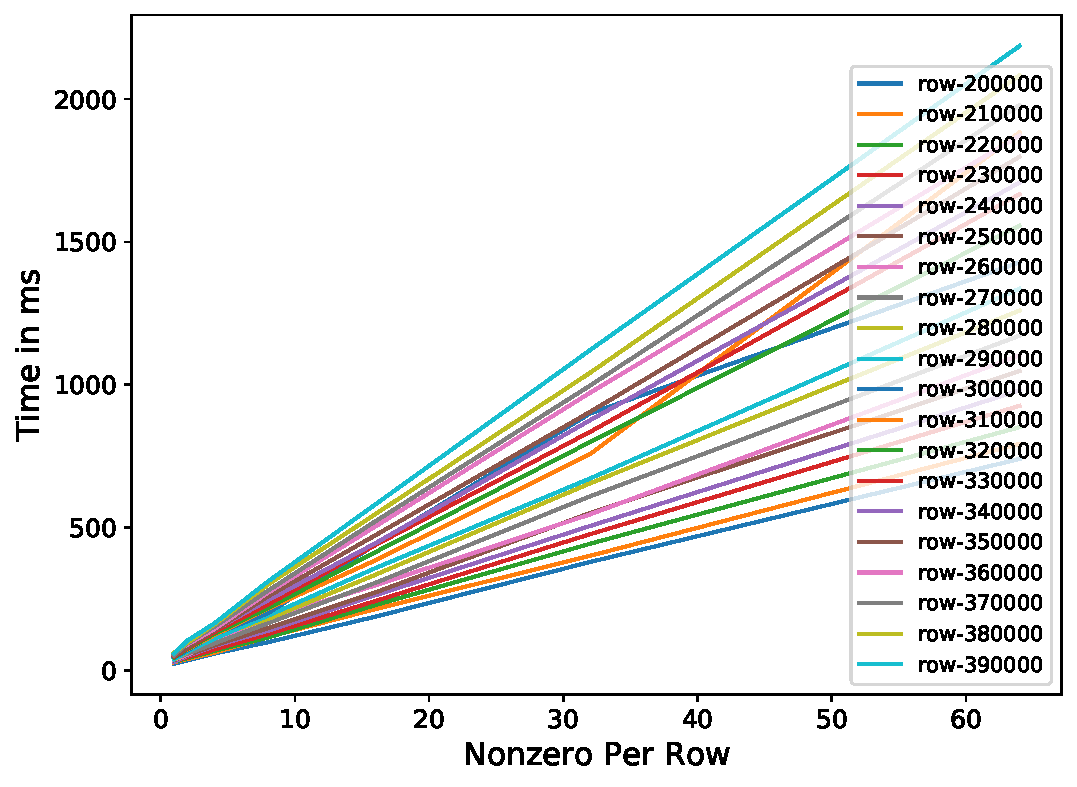
\includegraphics[width=0.48\linewidth]{figures/model_nonzero_perRow_for_particular_row_process_100.pdf}\label{fig:npr}}
\subfigure[Sample equation for the linear model.]{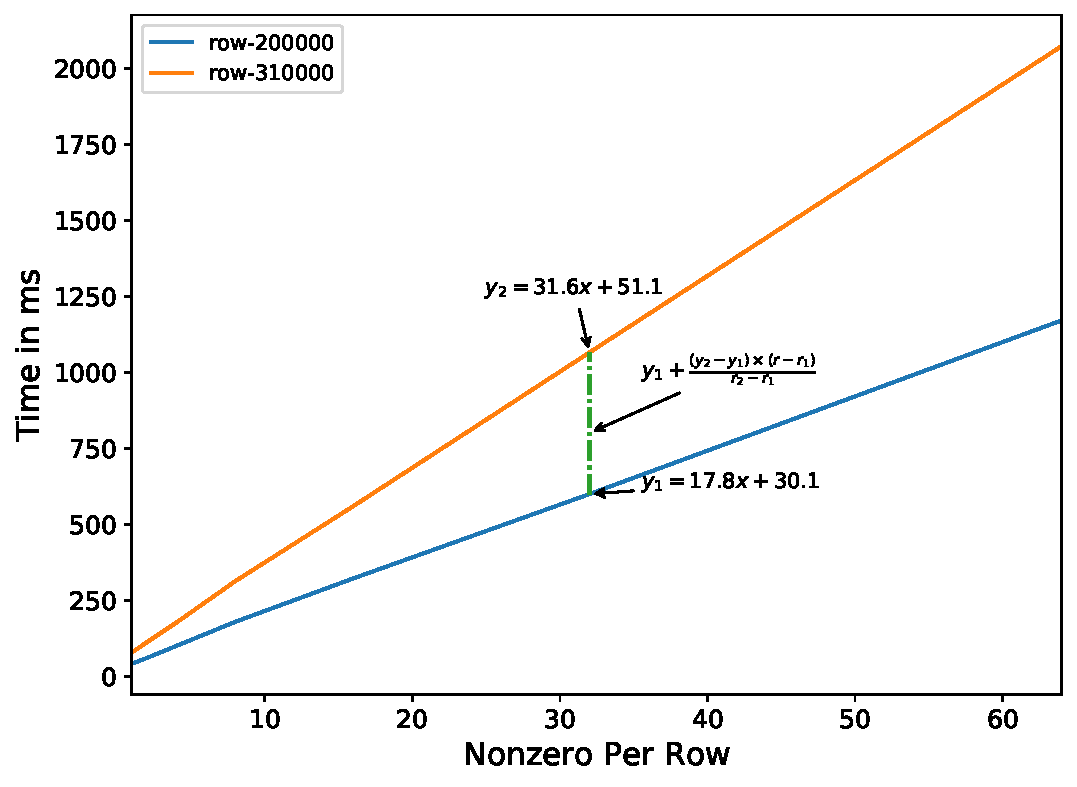
\includegraphics[width=0.48\linewidth]{figures/prediction_equation.pdf}\label{fig:linearspmvmodel}}
\caption{Linear relationship between nonzero per row and run time for the SpMV on the uniform 2d-Partitioning.}
\label{fig:ov-linear-model}
\end{figure}
Figure~\ref{fig:linearspmvmodel} shows the example for the matrix with $250000$ average rows per process and 32 nonzero per row. 
Here, possible $r_1$ and $r_2$ equations are available for rows $200000$ and $310000$. The figure reflects the prediction mechanism of our 
system. 


\subsection{Polynomial Support Vector Regression(SVR) Model}
\label{sec:svr-spmv}
We build the polynomial SVR model for all three algorithms
(\textit{2D-Uniform partitioning SpMV, G1DR-SpMV, and L1DR-SpMV}). The
performance of the SVR models largely depends on the appropriate
attributes for the model. Then choose the proper values for the
\textit{free parameters} of the SVR model.  \textit{Cross-Validation}
and \textit{Grid-Search} widely use to do that for the SVR model. The
models are built for a particular system, therefore they assume a
fixed number of processors and interconnect.

\subsubsection{Cross-Validation and Grid-Search}
Initially, we split the matrices into train and test data set, no test
data participate in the training mechanism. Here, we choose the
polynomial (``poly'') kernel to perform all the machine learning
regression. In this kernel, some free variables need to choose. 
There are no fixed values for these variables, based on the
application criteria it can vary. We select $5-fold$ cross-validation
that means we split the training set into 5 different parts, and among
5 parts we choose 4 as a training set and the remaining one as a test
set. In the grid search, one need to select a set of variables for the
free variable($C,\gamma$), like $C=\{2^{-2},
2^{-1}, \dots, 2^4, 2^5\}\text{ and }\gamma=\{0.01, 0.02, \dots, 0.2, 0.3\}$
and for each pair of variable need to perform cross-validation and
record the score. Then select a pair that gives the best performance
in cross-validation.  The next step is to train the model using the best
variable on the whole train set.

\subsubsection{Feature selection}
We build up polynomial support vector regression(SVR) models for three
different SpMV algorithms on the two different graph formats(CSR,
COO).  The SVR model follows the same mechanism for all multiplication
algorithm. The model predicts the average run time for a particular
test matrix based on its attributes. So, attributes are the key to a
good performance model.  Although the local multiplication is the same
for every algorithm, the communications are different for the
different partitioning modes. The common attributes for all three
algorithms are:

\begin{enumerate}
\label{list:static-attributes}
\item Average rows per process.
\item Average non zero per process.
\item Average non-zero per row.
\item Density of the matrix.
\item Standard deviation of the non zero per row.
\end{enumerate}

But the communication among the MPI process in the Local L1DR-SpMV
(one-to-one) is different than the other two(one-to-all or all-to-all).
That is why based on the sparsity of the matrices the communication
can vary a lot. For that, we need the following extra attributes for
the L1DR-SpMV which can be extracted after partitioning.

\begin{enumerate}
\item Average local non-zero elements.
\item Average global non-zero elements.
\item Average inter-process call.
\item Average data transfer.
\end{enumerate}

\subsection{SpMV Model from Micro-Benchmark}
In this model, we predict the runtime of the SPMV based the performance of couple of micro-benchmark of 
a selected computer architecture. Initially, SpMV on the distributed system can be divided into two main parts,
\begin{itemize}
\item Core Calculation: performance of the matrix-vector calculation in a MPI node.
\item MPI Communication: communication runtime among MPI ranks(processes). 
\end{itemize}
\subsubsection{Instruction Cost}
We can represent the basic SpMV by $y=y+Val*x$, which requires two floating point operation(multiply and addition). 
So, we can say we need to calculate NNZ(number of non-zeros) times FMA(fused multiply addition) to perform SpMV.
But, first it needs to load the data and SpMV is bound by the memory bandwidth rather than instruction. So, we 
separated the \textit{core calculation} into,
\begin{itemize}
\item Run time for FMA: $L_{FMA}\times NNZ$, where $L_{FMA}$ is the latency of a single FMA and $NNZ$ is number of non-zeros.
\item Memory access latency: $L_{RW}$
\end{itemize} 



\paragraph{Micro Benchmark for \textit{FMA}}
The throughput of SkylakeX is 2 instructions per cycle and the latency of FMA is 4 cycles. So there is a potential 
of pipelinling($2\times 4 = 8$) to get the optimal results. Now, SkylakeX 
has 512-bit register that can give the ability of the vectorization. For 64-bits floating point operation it can give vector 
width 8 and for 32-bits it can give at max vector width 16. To find the peak performance of the FMA and to avoid the 
read-write latency we need to setup the benchmark that datasets can be contained in the register. Now, SkylakeX has 32 
registers. We can populate the pipeline by using sufficient ampunt of work. By varying the 
number of fused-multiply-addition calculation, we can find out the performance limitation. From the information of the 
processors, we can say that 4 cycles required for \textit{FMA} and the throughput of the FMA is 2 instruction per cycle, that means 
we should at least use $4\times 2=8$ instruction at a time to populate the pipeline.
\begin{figure}[hbt!]
	\centering
	\subfigure[Vector Width: 4]{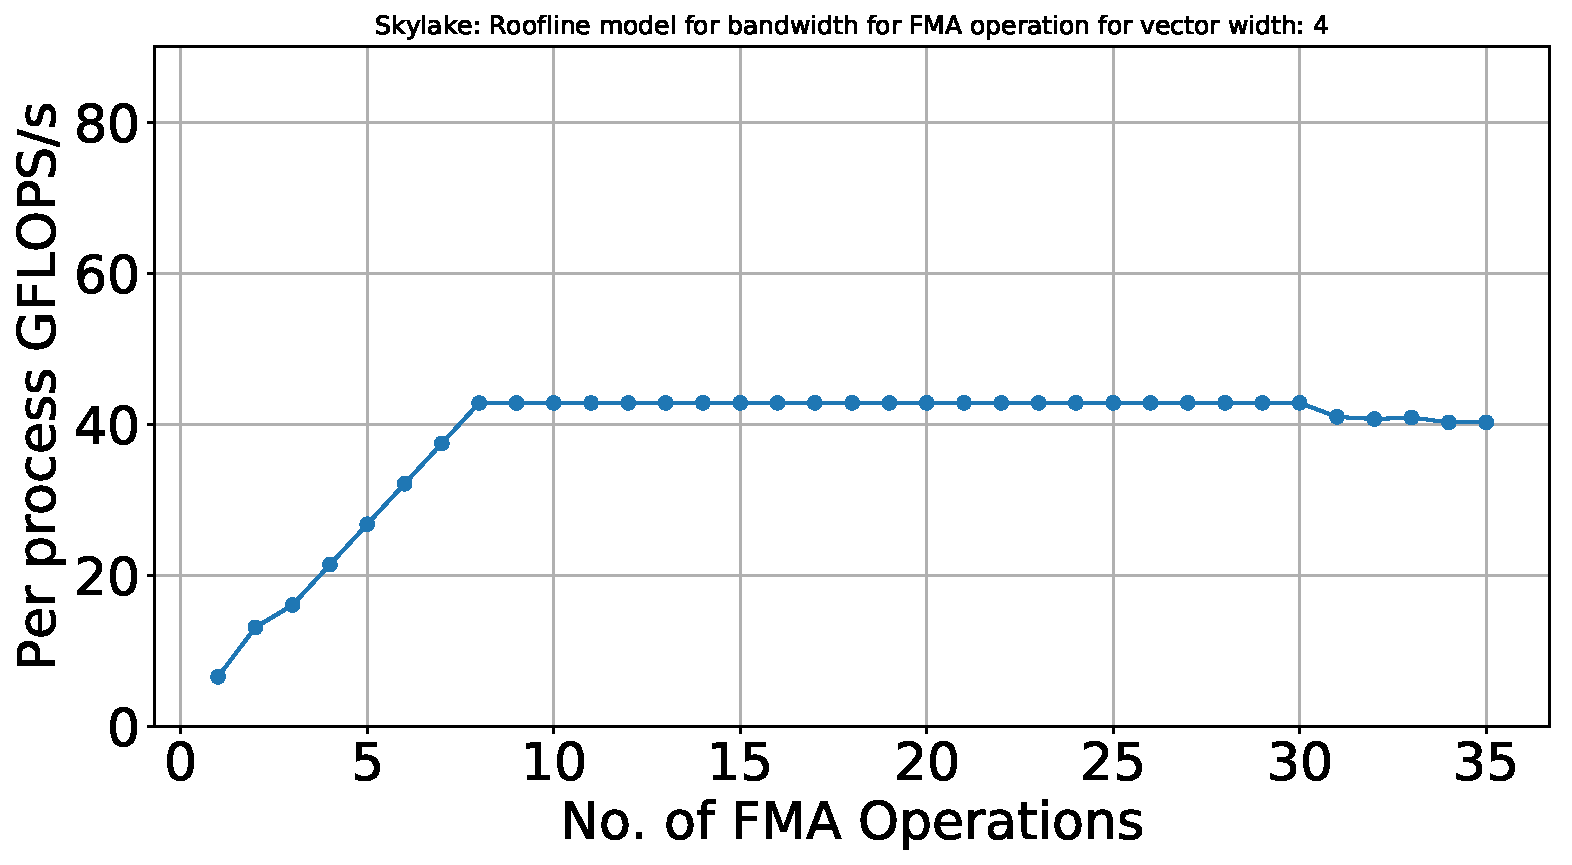
\includegraphics[width=0.48\linewidth]{figures/fma/skylake_mpi_fma_roofline_model_for_vec_4.pdf}		\label{fig:mpi-skl-vec-4}}
	\subfigure[Vector Width: 8]{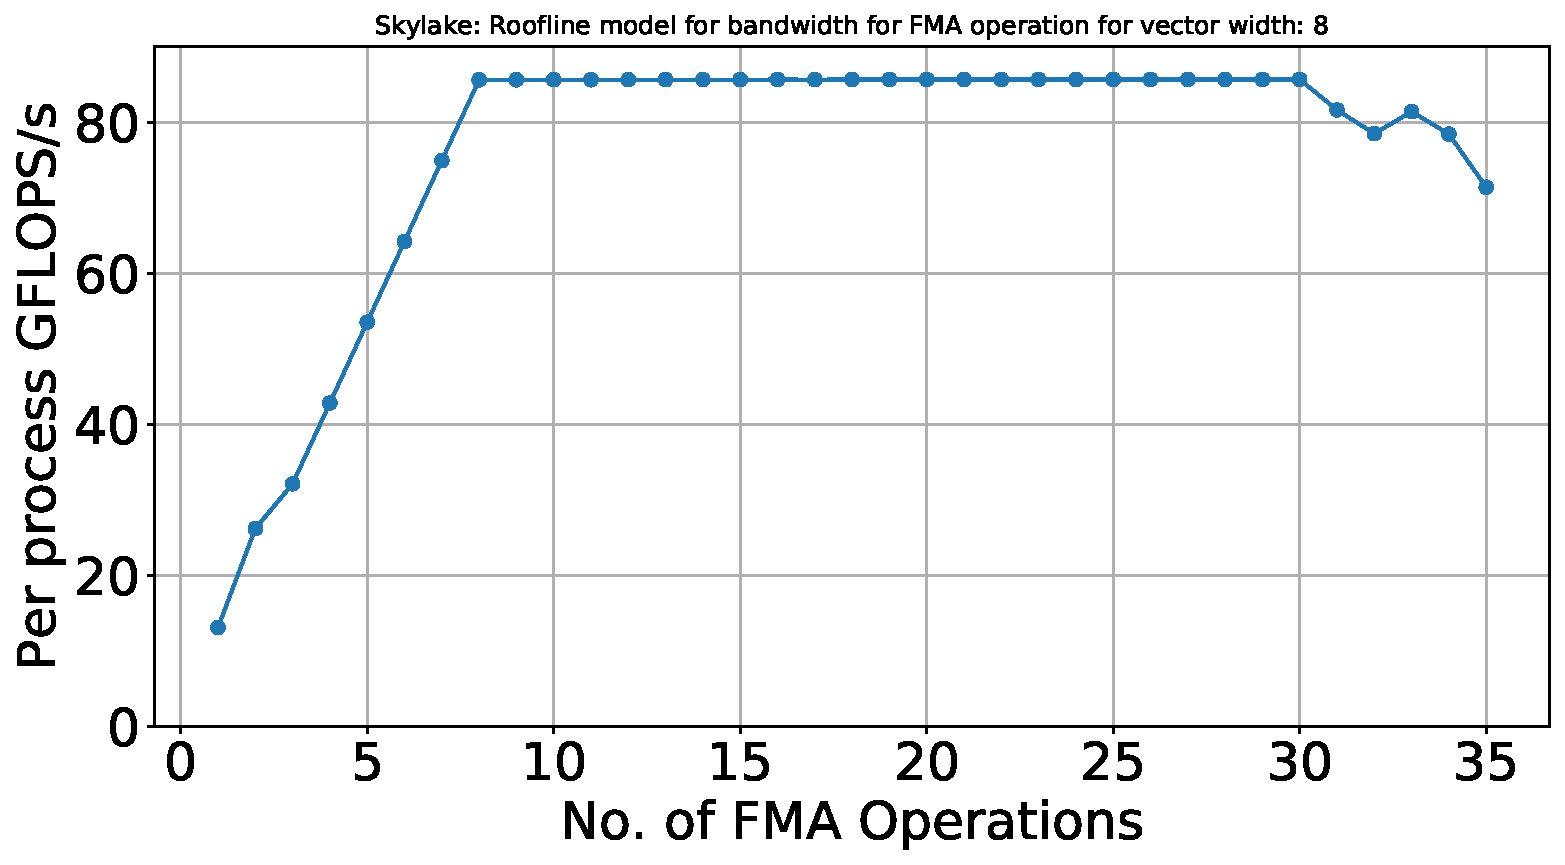
\includegraphics[width=0.48\linewidth]{figures/fma/skylake_mpi_fma_roofline_model_for_vec_8.pdf}		\label{fig:mpi-skl-vec-8}}
	\caption{Skylake: (MPI)Roofline model for bandwidth for FMA operation}
	\label{fig:mpi-skl-fma}
\end{figure}
Figure~\ref{fig:mpi-skl-fma} shows the roofline model of the \textit{FMA} on SkylakeX processor. 
We can estimate the theoritical peak performance a single FMA by the following equation,
\begin{eqnarray*}
P\ =\ Base\_Clock\_Frequency\times Vector\_Width\times \frac{FLOPs}{Instruction}
\end{eqnarray*}
The significance of the \textit{FMA} 
latency is actually negligible compare to the memory access latency. 

\subsubsection{Memory Accesses Cost}

\paragraph{Micro-Benchmark for Memory Access}
We use the \textit{STREAM}~\cite{mccalpin1995stream} benchmark to find
out the cost the memory accesses for a selected architecture.

\begin{figure}[hbt!]
	\centering
	\subfigure[Single Precision.]{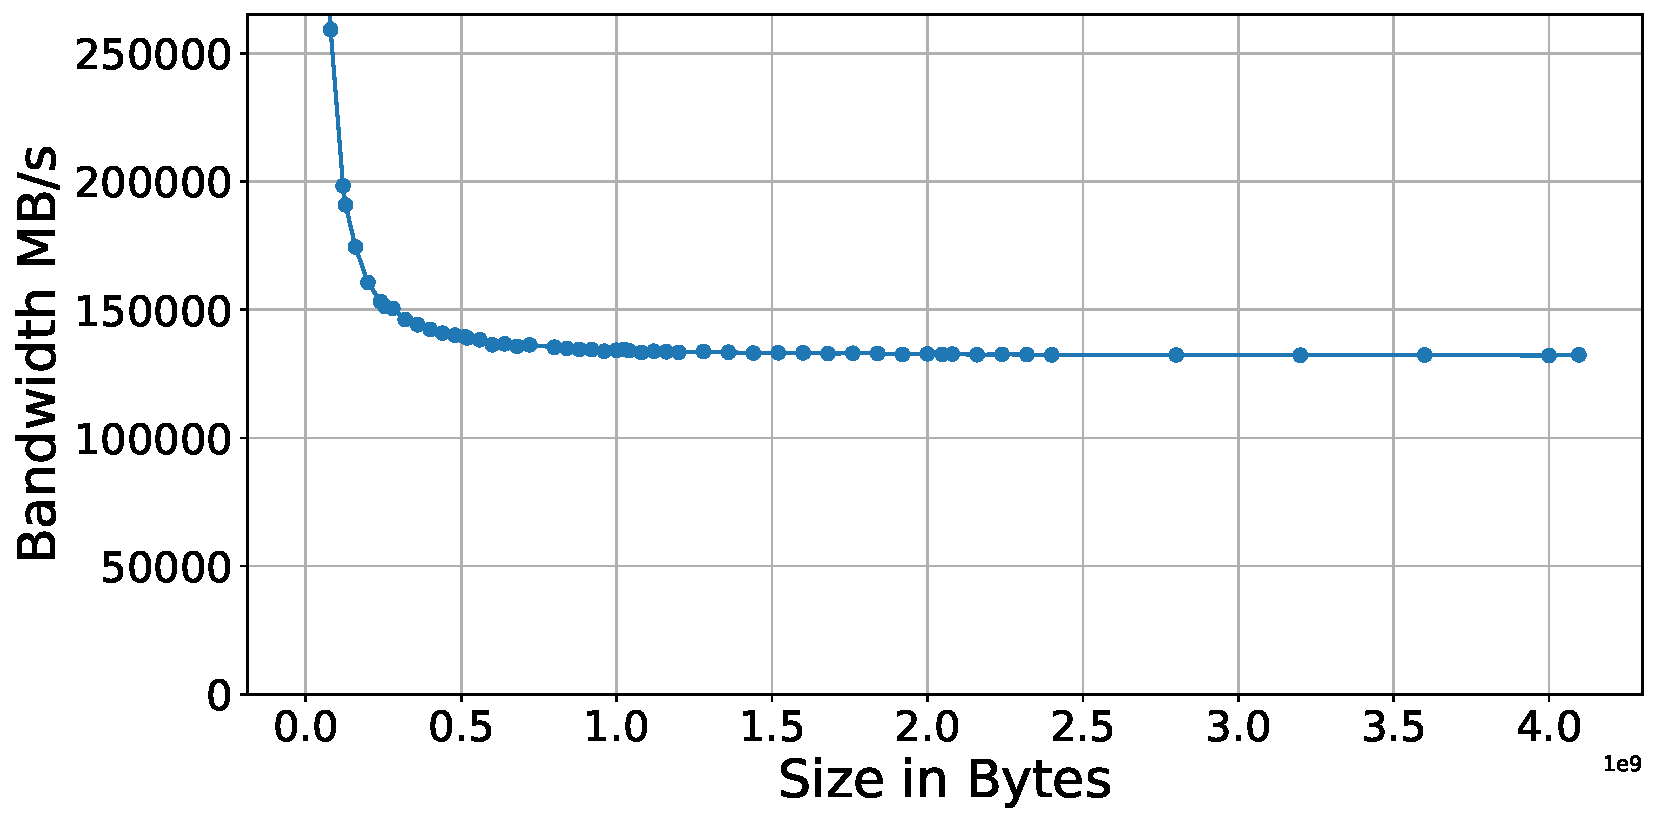
\includegraphics[width=0.48\linewidth]{figures/stream/skylake_mpi_copy_single_precision.pdf}		\label{fig:stream-single-copy}}
	\subfigure[Double Precision.]{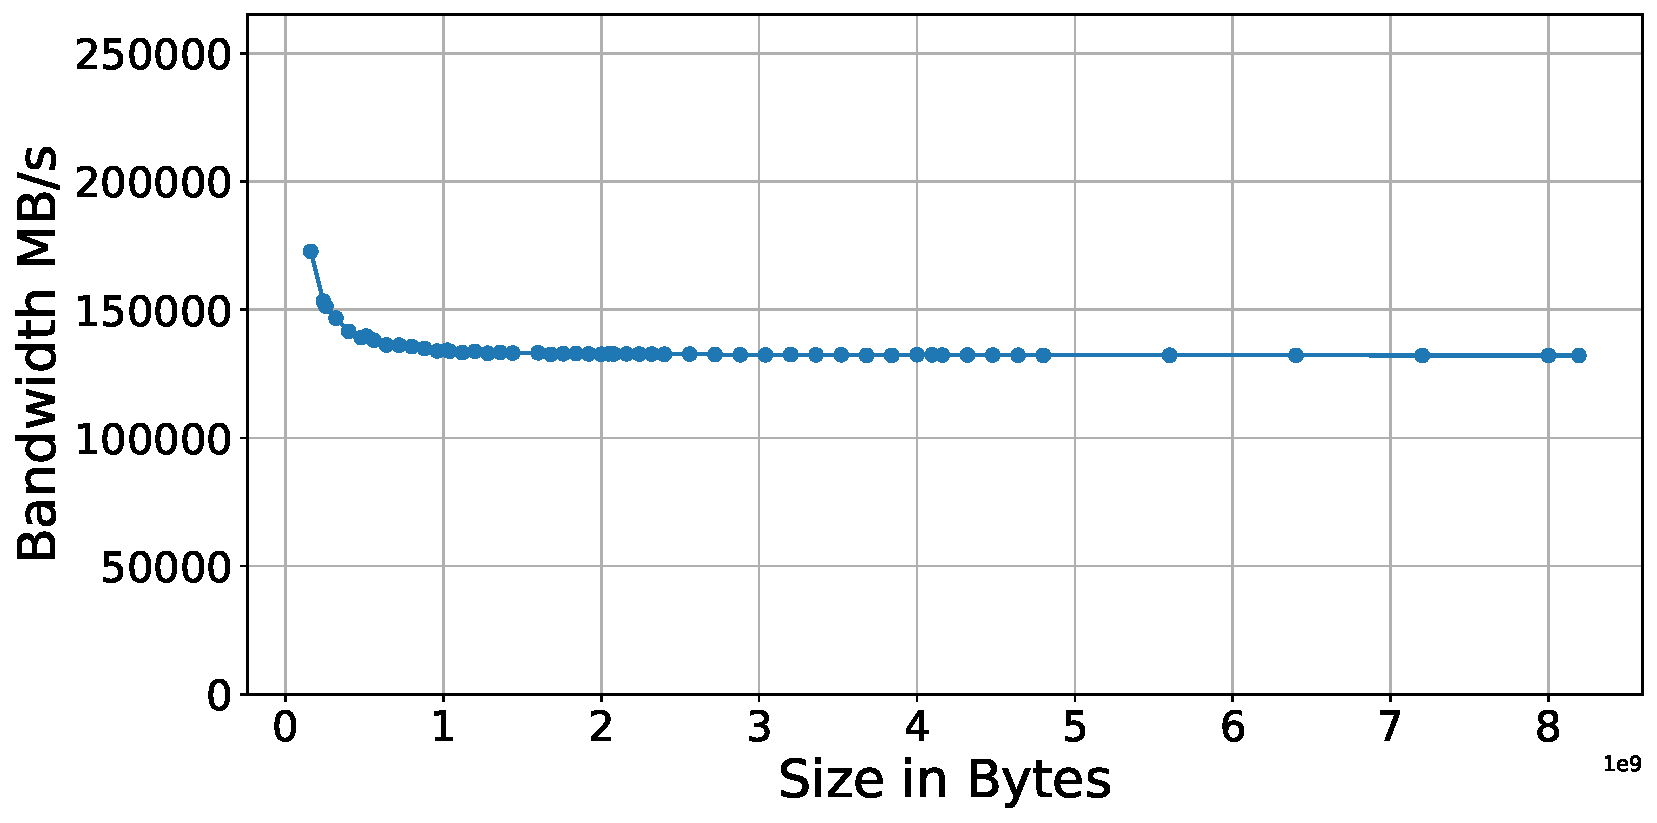
\includegraphics[width=0.48\linewidth]{figures/stream/skylake_mpi_copy_double_precision.pdf}		\label{fig:stream-double-copy}}
	\caption{Single and double precision memory access bandwidth on Skylake processor.}
	\label{fig:stream-copy-bandwidth}
\end{figure}

Figure~\ref{fig:stream-copy-bandwidth} shows the relation between data
size and bandwidth of the SkylakeX processor. To pick the right
bandwidth for a matrix-vector multiplication, we first calculate the
size of the data. Based on the size of the data, we pick the average
of the available immediate lower and higher point of the
benchmark. Note that in STREAM, all memory accesses are sequential.
 
\paragraph{Cache Access Patterns}
In SpMV some of the arrays are traverse sequentially and some have irregular
pattern. Table~\ref{tab:csr-spmv-2d-property} shows the memory access
property for different matrix representation format. We can see the
access to the vector \texttt{x} is irregular for both CSR and COO
format. But access to the vector \texttt{y} is only irregular for the
COO format.

One could model all irregular accesses as random accesses. However we
know that most graphs actually exhbit significant
locality~\cite{Beamer15}. We model the memory accesses by computing a
cache friendliness metric which represent the fraction of access that
are in cache and the fraction that are in memory.

This cache friendliness is computed for a matrix as follows. We assume
the matrix is traversed sequentially and we model the access to the
cache assuming the cache has the granularity of a cache line and that
the cache replacement policy is LRU. And we assume that the cache is
of the size of the L3 cache divided by the number of core on the
processor. This model does not accurately capture many properties of
the memory subsystem (such as associativity of caches, or cache
sharing across multiple cores, the fact that there are multiple levels
of caches, and concurrent processes); but it is a simple to compute
estimation of how irregular the memory access actually are.

All the sequential data accesses and \textit{hits} of irregular
accesses are treated as \textit{Sequential} data accesses. The cost of
these data accesses is accounted based on the predicted bandwidth to
the core out of the STREAM benchmark. And all cache \textit{miss} in
irregular accesses are treated to \texttt{Random} data accesses. The
cost of these operations are accounted based on the latency of the
memory access by the cores. The cost of these sequential and random
access are summed.

Note that this model does not capture all the complexity of modern
system: for instance, a mix of latency bound and bandwidth bound
memory operations can overlap especially when multiple cores access
memory at the same time. But while one could certainly craft an
example where the model is very inaccurate, we do not believe these
extreme case would happen in practice.

\begin{table}[htb]
\caption{Memory Access Property for 2D-Partitioning SpMV Model(RPP=rows per process, NNZ=non-zero elements).}
\label{tab:csr-spmv-2d-property}
\centering
\begin{tabular}[c]{| l | c | c | c | c | c |}
\hline
\multirow{2}{*}{Array} & \multicolumn{2}{ | c |}{Elements Size} & \multirow{2}{*}{Data Type} & \multicolumn{2}{ | c |}{Access Type} \\ \cline{2-3} \cline{5-6}
  &  CSR & COO  & &  CSR & COO \\ \hline
rowA & 2$\times$RPP & NNZ & Integer & Sequential & Sequential \\ \hline
colA & NNZ & NNZ & Integer & Sequential & Sequential  \\ \hline
valA & NNZ & NNZ & Floating & Sequential &  Sequential \\ \hline
x & NNZ  & NNZ & Floating & Irregular &  Irregular \\ \hline
y & RPP & NNZ & Floating & Sequential & Irregular  \\ \hline
\end{tabular}
\end{table}



\subsubsection{Micro-Benchmark for MPI communication}
MPI communications mostly depend on the size of the message and
network topology. We build a benchmark based on the OSU-MPI-Benchmark.
Because of the dynamics of the network topology we build a polynomial
model based on the number of nodes, number of MPI ranks, message size,
and MPI communication type. \todo{What does that mean. Is that an SVR model?}

\begin{comment}
\begin{figure}[hbt!]
	\centering
	\subfigure[MPI All\_GatherV.]{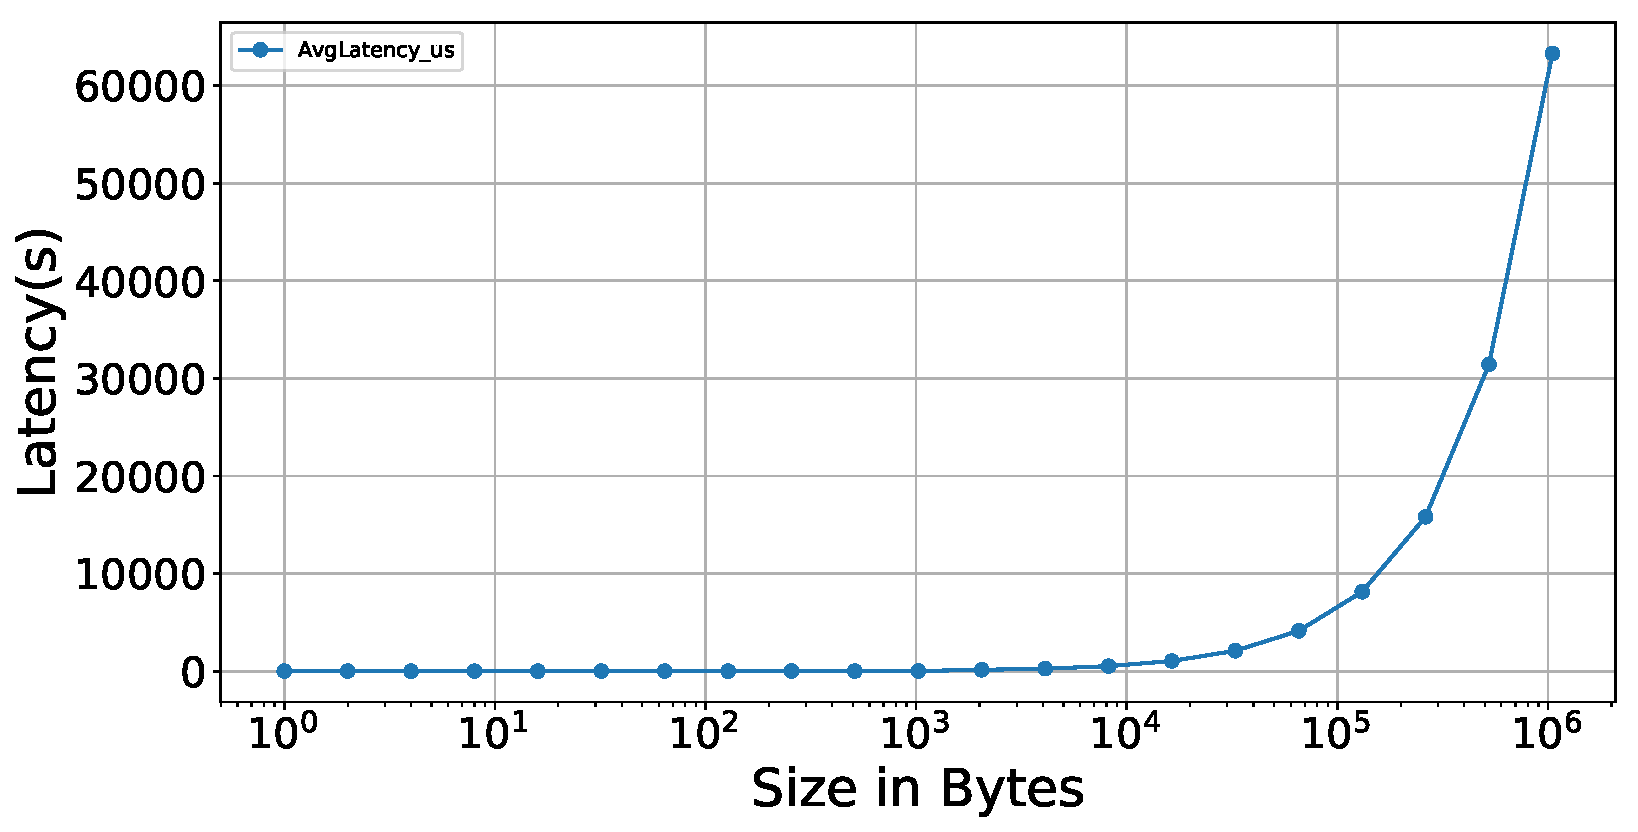
\includegraphics[width=0.48\linewidth]{figures/osu/skylake_mpi_allgatherv.pdf}		\label{fig:osu-skylake-allgatherv}}
	\subfigure[MPI All\_Reduce.]{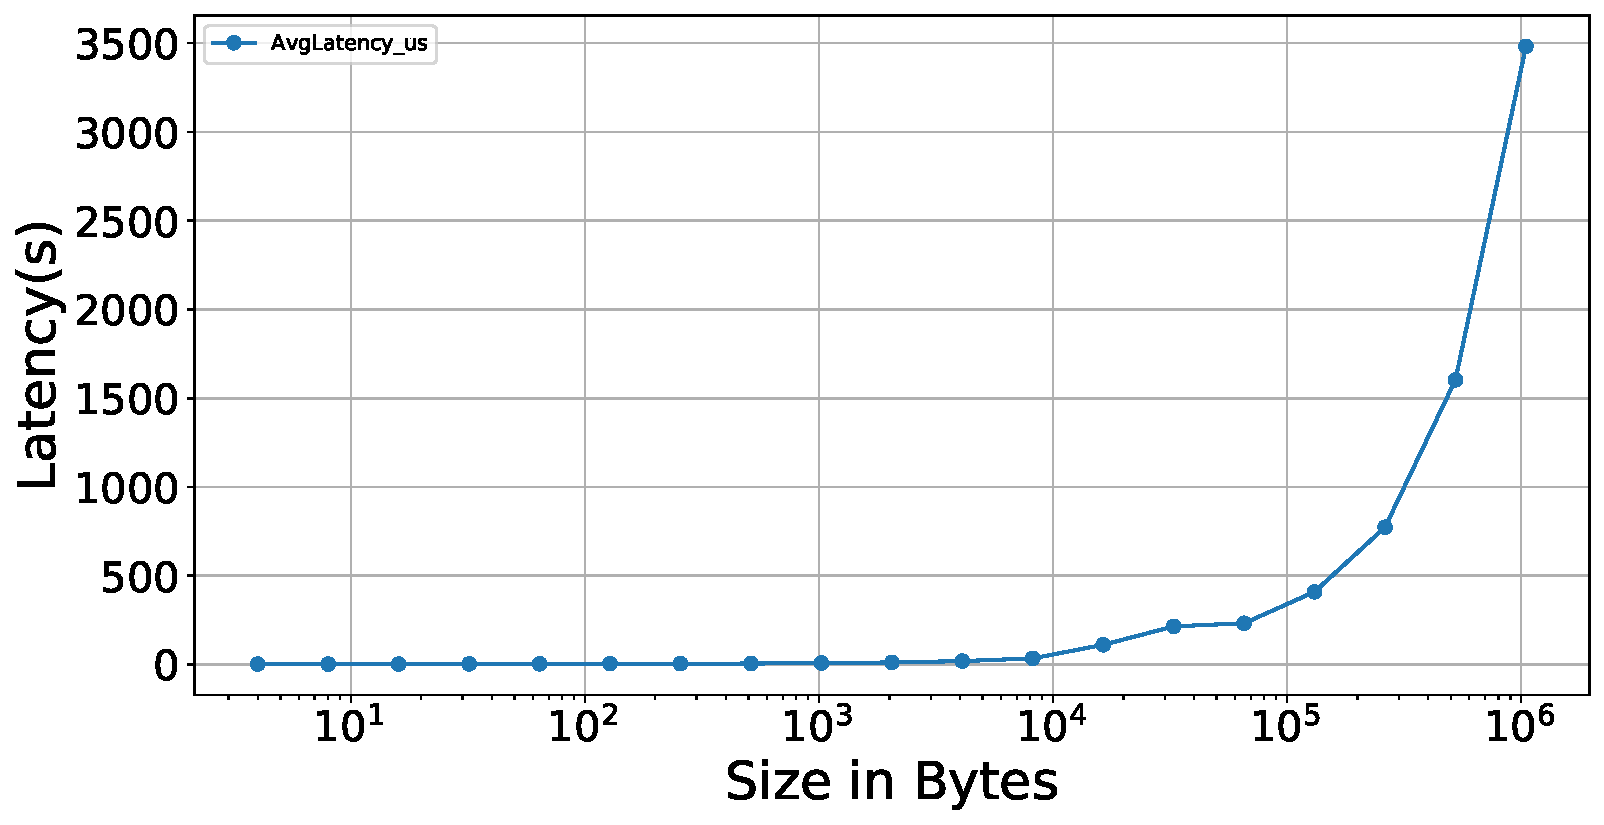
\includegraphics[width=0.48\linewidth]{figures/osu/skylake_mpi_allreduce.pdf}		\label{fig:osu-skylake-reduce}}
	\caption{Latency of the MPI collectives(All\_GatherV and All\_Reduce) on Skylake.}
	\label{fig:osu-collectives}
\end{figure}
\end{comment}

\subsubsection{Putting it together}

Figure~\ref{fig:spmv-model-from-benchmark} shows the overall structure of the SPMV model from micro-benchmark.

\begin{figure}[hbt!]
	\centering
	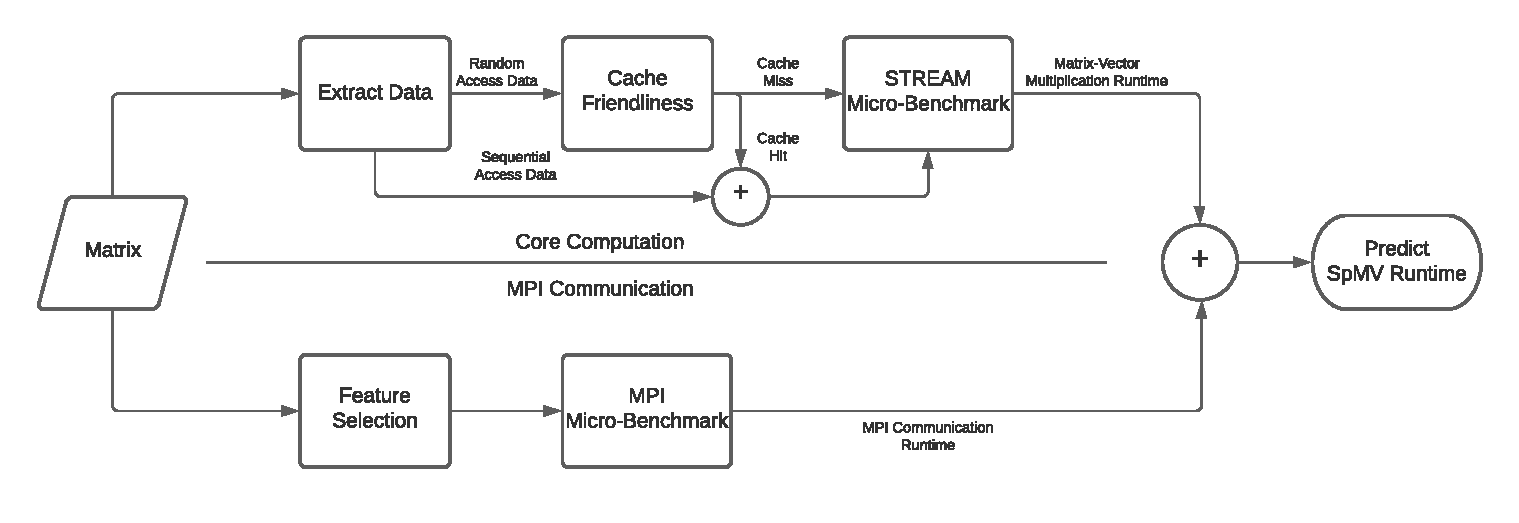
\includegraphics[width=0.96\linewidth]{figures/spmv_hardware_model.pdf}
	\caption{Structure of the SpMV model from micro-benchmark.}
	\label{fig:spmv-model-from-benchmark}
\end{figure}





\section{Experimental Settings}
\subsection{Hardware Platform and Operating System}
All the nodes of the computing cluster come with Intel Xeon Gold
6154 processors (SkylakeX architecture) and 388GB of DDR4
memory. Each node has 36 cores in 2 sockets. Hyper-threading is
disabled. The base frequency of each processor is 3.00 GHz.  Each
processor has 25 MB of L3 Cache. The nodes are connected by EDR
Infiniband. The machine uses the \texttt{Linux}. To present
concise results all experiments are performed on 144, 169, 225 and 256 MPI processes
allocated on 4, 5, 7 and 8 nodes respectively. The system support maximum 256 MPI processes.

\subsection{Matrices}

All the matrices we use come from the SuiteSparse Matrix Collection
(previously known as the \textit{Florida Sparse Matrix}
collection)~\cite{Davis11}. We used seven matrices for our
tests. Their properties are described in Table~\ref{tab:test_mat_info}.
\todo{make a table with stats of the matrices and reference it.}

Because the linear and SVR models require to be trained based on
timings from real runs, we used an other 83 matrices in order to train
these two models.

\begin{table}[htb]
\caption{Properties of the test matrices.}
\label{tab:test_mat_info}
\let\center\empty
\let\endcenter\relax
\centering
\resizebox{.8\width}{!}{\begin{tabular}[c]{| l | c | c | c |} 
\hline 
Name & Rows & Columns & Nonzero Elements \\ \hline
333SP & 3,712,815 & 3,712,815 & 22,217,266 \\ \hline
AS365 & 3,799,275 & 3,799,275 & 22,736,152 \\ \hline
M6 & 3,501,776 & 3,501,776 & 21,003,872 \\ \hline
NLR & 4,163,763 & 4,163,763 & 24,975,952 \\ \hline
hugetrace-00010 & 12,057,441 & 12,057,441 & 36,164,358 \\ \hline
road\_central & 14,081,816 & 14,081,816 & 33,866,826 \\ \hline
road\_usa & 23,947,347 & 23,947,347 & 57,708,624\\ \hline
\end{tabular}
}
\end{table}

\subsection{Results}

We will resent two types of results, runtimes on particular matrices
and number of MPI processes for a particular execution mode of
SpMV. We will also present relative errors for models calculated by:
\begin{eqnarray*}
error =\ \frac{actual\ time - predicted\ time}{actual\ time}\times 100
\end{eqnarray*}

\section{Experimental Results}

\subsection{Runtime of SpMV}

Table~\ref{} present the results of the different way of executing SpMV.

Looking first at the different 1D partitioning results. We can see
that having dedicated communication patterns to only access typically
delivers better performance than obtaining the complete



\subsection{SpMV Model from Micro-Benchmark}
\subsubsection{Random 2D-SpMV}
Table~\ref{tab:overall-spmv-csr-2d-single} and~\ref{tab:overall-spmv-coo-2d-single} shows the overall performance of the 
SpMV on the 2D-Partitioning model on CSR and COO storage formats respectively.  Average error for the CSR and COO formats are 
$7.62$ and $9.16$ respectively. The error is calculate by,

\begin{table}[htb]
\caption{Benchmark SpMV Model on Random CSR 2D Partitioning(on SkylakeX).}
\label{tab:overall-spmv-csr-2d-single}
\let\center\empty
\let\endcenter\relax
\centering
\resizebox{.8\width}{!}{\begin{tabular}[c]{| l | c | c | c | c | c |} 
\hline 
\multirow{2}{*}{Matrices} & \multirow{2}{*}{Nodes} & \multirow{2}{*}{Processes} & \multicolumn{2}{| c |}{Time(s)} & \multirow{2}{*}{Error\%} \\ \cline{4-5} 
  &  &  & Actual & Predicted &  \\ \hline 
\multirow{4}{*}{333SP}  & 4 & 144 & 7.2E-03 & 7.1E-03 & 1.7\% \\ \cline{2-6} 
 & 5 & 169 & 5.7E-03 & 6.2E-03 & 9.2\% \\ \cline{2-6} 
 & 7 & 225 & 4.7E-03 & 4.9E-03 & 3.9\% \\ \cline{2-6} 
 & 8 & 256 & 4.2E-03 & 4.3E-03 & 1.5\% \\ \hline 
\multirow{4}{*}{AS365}  & 4 & 144 & 7.4E-03 & 7.3E-03 & 1.2\% \\ \cline{2-6} 
 & 5 & 169 & 5.8E-03 & 6.4E-03 & 9.8\% \\ \cline{2-6} 
 & 7 & 225 & 4.7E-03 & 5.1E-03 & 8.3\% \\ \cline{2-6} 
 & 8 & 256 & 4.4E-03 & 4.4E-03 & 1.4\% \\ \hline 
\multirow{4}{*}{M6}  & 4 & 144 & 6.8E-03 & 6.6E-03 & 2.8\% \\ \cline{2-6} 
 & 5 & 169 & 5.3E-03 & 5.8E-03 & 9.3\% \\ \cline{2-6} 
 & 7 & 225 & 4.4E-03 & 4.6E-03 & 4.7\% \\ \cline{2-6} 
 & 8 & 256 & 4.0E-03 & 4.0E-03 & 0.3\% \\ \hline 
\multirow{4}{*}{NLR}  & 4 & 144 & 8.2E-03 & 8.2E-03 & 0.1\% \\ \cline{2-6} 
 & 5 & 169 & 6.5E-03 & 7.2E-03 & 11.4\% \\ \cline{2-6} 
 & 7 & 225 & 5.4E-03 & 5.7E-03 & 5.6\% \\ \cline{2-6} 
 & 8 & 256 & 4.8E-03 & 5.0E-03 & 3.9\% \\ \hline 
\multirow{4}{*}{hugetrace-00010}  & 4 & 144 & 2.3E-02 & 2.1E-02 & 8.2\% \\ \cline{2-6} 
 & 5 & 169 & 2.0E-02 & 1.9E-02 & 6.7\% \\ \cline{2-6} 
 & 7 & 225 & 1.7E-02 & 1.6E-02 & 10.1\% \\ \cline{2-6} 
 & 8 & 256 & 1.4E-02 & 1.4E-02 & 3.4\% \\ \hline 
\multirow{4}{*}{road\_road}  & 4 & 144 & 2.5E-02 & 2.3E-02 & 7.4\% \\ \cline{2-6} 
 & 5 & 169 & 2.2E-02 & 2.1E-02 & 3.5\% \\ \cline{2-6} 
 & 7 & 225 & 1.9E-02 & 1.7E-02 & 9.4\% \\ \cline{2-6} 
 & 8 & 256 & 1.5E-02 & 1.6E-02 & 2.4\% \\ \hline 
\multirow{4}{*}{road\_road}  & 4 & 144 & 3.6E-02 & 3.9E-02 & 9.0\% \\ \cline{2-6} 
 & 5 & 169 & 3.6E-02 & 3.6E-02 & 0.1\% \\ \cline{2-6} 
 & 7 & 225 & 3.1E-02 & 3.0E-02 & 3.1\% \\ \cline{2-6} 
 & 8 & 256 & 2.7E-02 & 2.7E-02 & 1.7\% \\ \hline 
\end{tabular} 
}

\end{table}

\begin{table}[htb]
\caption{Benchmark SpMV Model on Random COO 2D Partitioning(on SkylakeX).}
\label{tab:overall-spmv-coo-2d-single}
\let\center\empty
\let\endcenter\relax
\centering
\resizebox{.8\width}{!}{\begin{tabular}[c]{| l | c | c | c | c | c |} 
\hline 
\multirow{2}{*}{Matrices} & \multirow{2}{*}{Nodes} & \multirow{2}{*}{Processes} & \multicolumn{2}{| c |}{Time(s)} & \multirow{2}{*}{Error\%} \\ \cline{4-5} 
  &  &  & Actual & Predicted &  \\ \hline 
\multirow{4}{*}{333SP}  & 4 & 144 & 5.4E-03 & 5.6E-03 & 3.7\% \\ \cline{2-6} 
 & 5 & 169 & 4.2E-03 & 5.0E-03 & 19.6\% \\ \cline{2-6} 
 & 7 & 225 & 3.5E-03 & 4.0E-03 & 15.5\% \\ \cline{2-6} 
 & 8 & 256 & 3.4E-03 & 3.5E-03 & 4.3\% \\ \hline 
\multirow{4}{*}{AS365}  & 4 & 144 & 5.5E-03 & 5.8E-03 & 4.0\% \\ \cline{2-6} 
 & 5 & 169 & 4.3E-03 & 5.1E-03 & 19.7\% \\ \cline{2-6} 
 & 7 & 225 & 3.6E-03 & 4.1E-03 & 13.6\% \\ \cline{2-6} 
 & 8 & 256 & 3.6E-03 & 3.6E-03 & 0.1\% \\ \hline 
\multirow{4}{*}{M6}  & 4 & 144 & 5.0E-03 & 5.2E-03 & 3.5\% \\ \cline{2-6} 
 & 5 & 169 & 3.9E-03 & 4.6E-03 & 18.7\% \\ \cline{2-6} 
 & 7 & 225 & 3.4E-03 & 3.8E-03 & 9.7\% \\ \cline{2-6} 
 & 8 & 256 & 3.3E-03 & 3.3E-03 & 0.8\% \\ \hline 
\multirow{4}{*}{NLR}  & 4 & 144 & 6.1E-03 & 6.4E-03 & 4.9\% \\ \cline{2-6} 
 & 5 & 169 & 4.8E-03 & 5.7E-03 & 19.6\% \\ \cline{2-6} 
 & 7 & 225 & 4.0E-03 & 4.6E-03 & 15.2\% \\ \cline{2-6} 
 & 8 & 256 & 3.9E-03 & 4.0E-03 & 2.8\% \\ \hline 
\multirow{4}{*}{hugetrace-00010}  & 4 & 144 & 1.7E-02 & 1.6E-02 & 4.2\% \\ \cline{2-6} 
 & 5 & 169 & 1.3E-02 & 1.5E-02 & 13.7\% \\ \cline{2-6} 
 & 7 & 225 & 1.1E-02 & 1.2E-02 & 9.5\% \\ \cline{2-6} 
 & 8 & 256 & 1.0E-02 & 1.1E-02 & 9.2\% \\ \hline 
\multirow{4}{*}{road\_central}  & 4 & 144 & 1.9E-02 & 1.8E-02 & 5.6\% \\ \cline{2-6} 
 & 5 & 169 & 1.5E-02 & 1.7E-02 & 12.4\% \\ \cline{2-6} 
 & 7 & 225 & 1.3E-02 & 1.4E-02 & 8.7\% \\ \cline{2-6} 
 & 8 & 256 & 1.2E-02 & 1.3E-02 & 8.1\% \\ \hline 
\multirow{4}{*}{road\_usa}  & 4 & 144 & 2.9E-02 & 3.0E-02 & 3.7\% \\ \cline{2-6} 
 & 5 & 169 & 3.2E-02 & 2.8E-02 & 12.6\% \\ \cline{2-6} 
 & 7 & 225 & 2.3E-02 & 2.4E-02 & 5.4\% \\ \cline{2-6} 
 & 8 & 256 & 2.0E-02 & 2.2E-02 & 7.6\% \\ \hline 
\end{tabular} 
}
\end{table}

\subsubsection{Local 1D-SpMV}
Table~\ref{tab:overall-spmv-csr-lk-single} and~\ref{tab:overall-spmv-coo-lk-single} shows the overall performance of the Local 1D-Partitioning 
SpMV model on CSR and COO storage formats respectively.  Average error for the CSR and COO formats are 
$21.61$ and $19.52$ respectively. 

\begin{table}[htb]
\caption{Benchmark SpMV Model on Local CSR 1D-Row Partitioning(on SkylakeX).}
\label{tab:overall-spmv-csr-lk-single}
\let\center\empty
\let\endcenter\relax
\centering
\resizebox{.8\width}{!}{\begin{tabular}[c]{| l | c | c | c | c | c |} 
\hline 
\multirow{2}{*}{Matrices} & \multirow{2}{*}{Nodes} & \multirow{2}{*}{Processes} & \multicolumn{2}{| c |}{Time(s)} & \multirow{2}{*}{Error\%} \\ \cline{4-5} 
  &  &  & Actual & Predicted &  \\ \hline 
\multirow{4}{*}{333SP}  & 4 & 144 & 1.2E-03 & 1.2E-03 & 2.3\% \\ \cline{2-6} 
 & 5 & 169 & 1.1E-03 & 1.1E-03 & 0.2\% \\ \cline{2-6} 
 & 7 & 225 & 8.4E-04 & 8.1E-04 & 3.8\% \\ \cline{2-6} 
 & 8 & 256 & 8.2E-04 & 7.4E-04 & 10.7\% \\ \hline 
\multirow{4}{*}{AS365}  & 4 & 144 & 1.3E-03 & 1.3E-03 & 3.9\% \\ \cline{2-6} 
 & 5 & 169 & 1.1E-03 & 1.1E-03 & 3.4\% \\ \cline{2-6} 
 & 7 & 225 & 9.2E-04 & 8.5E-04 & 7.5\% \\ \cline{2-6} 
 & 8 & 256 & 8.5E-04 & 7.8E-04 & 8.5\% \\ \hline 
\multirow{4}{*}{M6}  & 4 & 144 & 1.3E-03 & 1.2E-03 & 4.9\% \\ \cline{2-6} 
 & 5 & 169 & 1.1E-03 & 1.0E-03 & 2.9\% \\ \cline{2-6} 
 & 7 & 225 & 8.7E-04 & 7.9E-04 & 8.8\% \\ \cline{2-6} 
 & 8 & 256 & 8.3E-04 & 7.3E-04 & 12.0\% \\ \hline 
\multirow{4}{*}{NLR}  & 4 & 144 & 1.4E-03 & 1.4E-03 & 2.2\% \\ \cline{2-6} 
 & 5 & 169 & 1.3E-03 & 1.2E-03 & 5.4\% \\ \cline{2-6} 
 & 7 & 225 & 9.9E-04 & 9.3E-04 & 6.0\% \\ \cline{2-6} 
 & 8 & 256 & 9.5E-04 & 8.5E-04 & 10.4\% \\ \hline 
\multirow{4}{*}{hugetrace-00010}  & 4 & 144 & 2.5E-03 & 2.7E-03 & 8.2\% \\ \cline{2-6} 
 & 5 & 169 & 2.2E-03 & 2.4E-03 & 10.8\% \\ \cline{2-6} 
 & 7 & 225 & 1.8E-03 & 1.9E-03 & 7.8\% \\ \cline{2-6} 
 & 8 & 256 & 1.6E-03 & 1.7E-03 & 6.4\% \\ \hline 
\multirow{4}{*}{road\_central}  & 4 & 144 & 2.6E-03 & 2.9E-03 & 10.5\% \\ \cline{2-6} 
 & 5 & 169 & 2.4E-03 & 2.6E-03 & 9.0\% \\ \cline{2-6} 
 & 7 & 225 & 1.9E-03 & 2.1E-03 & 6.6\% \\ \cline{2-6} 
 & 8 & 256 & 1.8E-03 & 1.9E-03 & 6.0\% \\ \hline 
\multirow{4}{*}{road\_usa}  & 4 & 144 & 4.1E-03 & 4.1E-03 & 1.3\% \\ \cline{2-6} 
 & 5 & 169 & 3.4E-03 & 3.7E-03 & 6.1\% \\ \cline{2-6} 
 & 7 & 225 & 2.8E-03 & 3.0E-03 & 6.8\% \\ \cline{2-6} 
 & 8 & 256 & 2.6E-03 & 2.8E-03 & 9.7\% \\ \hline 
\end{tabular} 
}
\end{table}

\begin{table}[htb]
\caption{Benchmark SpMV Model on Local COO 1D-Row Partitioning(on SkylakeX).}
\label{tab:overall-spmv-coo-lk-single}
\let\center\empty
\let\endcenter\relax
\centering
\resizebox{.8\width}{!}{\begin{tabular}[c]{| l | c | c | c | c | c |} 
\hline 
\multirow{2}{*}{Matrices} & \multirow{2}{*}{Nodes} & \multirow{2}{*}{Processes} & \multicolumn{2}{| c |}{Time(s)} & \multirow{2}{*}{Error\%} \\ \cline{4-5} 
  &  &  & Actual & Predicted &  \\ \hline 
\multirow{4}{*}{333SP}  & 4 & 144 & 1.2E-03 & 1.2E-03 & 2.3\% \\ \cline{2-6} 
 & 5 & 169 & 1.1E-03 & 1.1E-03 & 0.2\% \\ \cline{2-6} 
 & 7 & 225 & 8.4E-04 & 8.1E-04 & 3.8\% \\ \cline{2-6} 
 & 8 & 256 & 8.2E-04 & 7.4E-04 & 10.7\% \\ \hline 
\multirow{4}{*}{AS365}  & 4 & 144 & 1.3E-03 & 1.3E-03 & 3.9\% \\ \cline{2-6} 
 & 5 & 169 & 1.1E-03 & 1.1E-03 & 3.4\% \\ \cline{2-6} 
 & 7 & 225 & 9.2E-04 & 8.5E-04 & 7.5\% \\ \cline{2-6} 
 & 8 & 256 & 8.5E-04 & 7.8E-04 & 8.5\% \\ \hline 
\multirow{4}{*}{M6}  & 4 & 144 & 1.3E-03 & 1.2E-03 & 4.9\% \\ \cline{2-6} 
 & 5 & 169 & 1.1E-03 & 1.0E-03 & 2.9\% \\ \cline{2-6} 
 & 7 & 225 & 8.7E-04 & 7.9E-04 & 8.8\% \\ \cline{2-6} 
 & 8 & 256 & 8.3E-04 & 7.3E-04 & 12.0\% \\ \hline 
\multirow{4}{*}{NLR}  & 4 & 144 & 1.4E-03 & 1.4E-03 & 2.2\% \\ \cline{2-6} 
 & 5 & 169 & 1.3E-03 & 1.2E-03 & 5.4\% \\ \cline{2-6} 
 & 7 & 225 & 9.9E-04 & 9.3E-04 & 6.0\% \\ \cline{2-6} 
 & 8 & 256 & 9.5E-04 & 8.5E-04 & 10.4\% \\ \hline 
\multirow{4}{*}{hugetrace-00010}  & 4 & 144 & 2.5E-03 & 2.7E-03 & 8.2\% \\ \cline{2-6} 
 & 5 & 169 & 2.2E-03 & 2.4E-03 & 10.8\% \\ \cline{2-6} 
 & 7 & 225 & 1.8E-03 & 1.9E-03 & 7.8\% \\ \cline{2-6} 
 & 8 & 256 & 1.6E-03 & 1.7E-03 & 6.4\% \\ \hline 
\multirow{4}{*}{road\_central}  & 4 & 144 & 2.6E-03 & 2.9E-03 & 10.5\% \\ \cline{2-6} 
 & 5 & 169 & 2.4E-03 & 2.6E-03 & 9.0\% \\ \cline{2-6} 
 & 7 & 225 & 1.9E-03 & 2.1E-03 & 6.6\% \\ \cline{2-6} 
 & 8 & 256 & 1.8E-03 & 1.9E-03 & 6.0\% \\ \hline 
\multirow{4}{*}{road\_usa}  & 4 & 144 & 4.1E-03 & 4.1E-03 & 1.3\% \\ \cline{2-6} 
 & 5 & 169 & 3.4E-03 & 3.7E-03 & 6.1\% \\ \cline{2-6} 
 & 7 & 225 & 2.8E-03 & 3.0E-03 & 6.8\% \\ \cline{2-6} 
 & 8 & 256 & 2.6E-03 & 2.8E-03 & 9.7\% \\ \hline 
\end{tabular} 
}
\end{table}


\subsubsection{Local 1D-SpMV}
Table~\ref{tab:overall-spmv-csr-gk-single} and~\ref{tab:overall-spmv-coo-gk-single} shows the overall performance of the Global 1D-Partitioning 
SpMV model on CSR and COO storage formats respectively.  Average error for the CSR and COO formats are 
$13.63$ and $25.3$ respectively. 

\begin{table}[htb]
\caption{Benchmark SpMV Model on Global CSR 1D-Row Partitioning(on SkylakeX).}
\label{tab:overall-spmv-csr-gk-single}
\let\center\empty
\let\endcenter\relax
\centering
\resizebox{.8\width}{!}{\begin{tabular}[c]{| l | c | c | c | c | c |} 
\hline 
\multirow{2}{*}{Matrices} & \multirow{2}{*}{Nodes} & \multirow{2}{*}{Processes} & \multicolumn{2}{| c |}{Time(s)} & \multirow{2}{*}{Error\%} \\ \cline{4-5} 
  &  &  & Actual & Predicted &  \\ \hline 
\multirow{4}{*}{333SP}  & 4 & 144 & 2.6E-02 & 2.1E-02 & 19.2\% \\ \cline{2-6} 
 & 5 & 169 & 2.0E-02 & 2.0E-02 & 2.2\% \\ \cline{2-6} 
 & 7 & 225 & 1.9E-02 & 1.8E-02 & 5.6\% \\ \cline{2-6} 
 & 8 & 256 & 2.4E-02 & 1.9E-02 & 21.2\% \\ \hline 
\multirow{4}{*}{AS365}  & 4 & 144 & 2.7E-02 & 2.2E-02 & 19.2\% \\ \cline{2-6} 
 & 5 & 169 & 2.1E-02 & 2.0E-02 & 2.7\% \\ \cline{2-6} 
 & 7 & 225 & 2.0E-02 & 1.9E-02 & 4.8\% \\ \cline{2-6} 
 & 8 & 256 & 2.4E-02 & 1.9E-02 & 21.2\% \\ \hline 
\multirow{4}{*}{M6}  & 4 & 144 & 2.5E-02 & 2.0E-02 & 19.2\% \\ \cline{2-6} 
 & 5 & 169 & 1.9E-02 & 1.8E-02 & 3.2\% \\ \cline{2-6} 
 & 7 & 225 & 1.8E-02 & 1.7E-02 & 4.5\% \\ \cline{2-6} 
 & 8 & 256 & 2.2E-02 & 1.8E-02 & 21.1\% \\ \hline 
\multirow{4}{*}{NLR}  & 4 & 144 & 2.9E-02 & 2.4E-02 & 19.1\% \\ \cline{2-6} 
 & 5 & 169 & 2.2E-02 & 2.2E-02 & 2.3\% \\ \cline{2-6} 
 & 7 & 225 & 2.1E-02 & 2.1E-02 & 4.1\% \\ \cline{2-6} 
 & 8 & 256 & 2.6E-02 & 2.1E-02 & 21.3\% \\ \hline 
\multirow{4}{*}{hugetrace-00010}  & 4 & 144 & 8.2E-02 & 6.6E-02 & 20.0\% \\ \cline{2-6} 
 & 5 & 169 & 6.2E-02 & 6.1E-02 & 0.7\% \\ \cline{2-6} 
 & 7 & 225 & 6.4E-02 & 5.7E-02 & 10.2\% \\ \cline{2-6} 
 & 8 & 256 & 7.3E-02 & 5.7E-02 & 22.7\% \\ \hline 
\multirow{4}{*}{road\_road}  & 4 & 144 & 9.6E-02 & 7.6E-02 & 20.2\% \\ \cline{2-6} 
 & 5 & 169 & 7.1E-02 & 7.1E-02 & 0.6\% \\ \cline{2-6} 
 & 7 & 225 & 7.4E-02 & 6.6E-02 & 10.3\% \\ \cline{2-6} 
 & 8 & 256 & 8.6E-02 & 6.6E-02 & 23.4\% \\ \hline 
\multirow{4}{*}{road\_road}  & 4 & 144 & 1.6E-01 & 1.3E-01 & 19.3\% \\ \cline{2-6} 
 & 5 & 169 & 9.9E-02 & 1.2E-01 & 23.8\% \\ \cline{2-6} 
 & 7 & 225 & 9.8E-02 & 1.1E-01 & 16.5\% \\ \cline{2-6} 
 & 8 & 256 & 1.5E-01 & 1.1E-01 & 23.0\% \\ \hline 
\end{tabular} 
}
\end{table}

\begin{table}[htb]
\caption{Benchmark SpMV Model on Global COO 1D-Row Partitioning(on SkylakeX).}
\label{tab:overall-spmv-coo-gk-single}
\let\center\empty
\let\endcenter\relax
\centering
\resizebox{.8\width}{!}{\begin{tabular}[c]{| l | c | c | c | c | c |} 
\hline 
\multirow{2}{*}{Matrices} & \multirow{2}{*}{Nodes} & \multirow{2}{*}{Processes} & \multicolumn{2}{| c |}{Time(s)} & \multirow{2}{*}{Error\%} \\ \cline{4-5} 
  &  &  & Actual & Predicted &  \\ \hline 
\multirow{4}{*}{333SP}  & 4 & 144 & 3.3E-02 & 2.1E-02 & 34.4\% \\ \cline{2-6} 
 & 5 & 169 & 2.7E-02 & 2.0E-02 & 26.0\% \\ \cline{2-6} 
 & 7 & 225 & 2.4E-02 & 1.9E-02 & 23.9\% \\ \cline{2-6} 
 & 8 & 256 & 2.7E-02 & 1.9E-02 & 30.9\% \\ \hline 
\multirow{4}{*}{AS365}  & 4 & 144 & 3.3E-02 & 2.2E-02 & 34.4\% \\ \cline{2-6} 
 & 5 & 169 & 2.7E-02 & 2.0E-02 & 26.1\% \\ \cline{2-6} 
 & 7 & 225 & 2.5E-02 & 1.9E-02 & 24.3\% \\ \cline{2-6} 
 & 8 & 256 & 2.8E-02 & 1.9E-02 & 31.0\% \\ \hline 
\multirow{4}{*}{M6}  & 4 & 144 & 3.1E-02 & 2.0E-02 & 35.2\% \\ \cline{2-6} 
 & 5 & 169 & 2.5E-02 & 1.9E-02 & 26.1\% \\ \cline{2-6} 
 & 7 & 225 & 2.3E-02 & 1.7E-02 & 23.9\% \\ \cline{2-6} 
 & 8 & 256 & 2.6E-02 & 1.8E-02 & 30.9\% \\ \hline 
\multirow{4}{*}{NLR}  & 4 & 144 & 3.6E-02 & 2.4E-02 & 34.5\% \\ \cline{2-6} 
 & 5 & 169 & 3.0E-02 & 2.2E-02 & 26.1\% \\ \cline{2-6} 
 & 7 & 225 & 2.7E-02 & 2.1E-02 & 24.1\% \\ \cline{2-6} 
 & 8 & 256 & 3.0E-02 & 2.1E-02 & 31.1\% \\ \hline 
\multirow{4}{*}{hugetrace-00010}  & 4 & 144 & 9.3E-02 & 6.6E-02 & 28.6\% \\ \cline{2-6} 
 & 5 & 169 & 6.7E-02 & 6.2E-02 & 7.6\% \\ \cline{2-6} 
 & 7 & 225 & 7.0E-02 & 5.7E-02 & 18.3\% \\ \cline{2-6} 
 & 8 & 256 & 7.9E-02 & 5.7E-02 & 28.2\% \\ \hline 
\multirow{4}{*}{road\_road}  & 4 & 144 & 1.1E-01 & 7.7E-02 & 27.1\% \\ \cline{2-6} 
 & 5 & 169 & 7.1E-02 & 7.2E-02 & 1.7\% \\ \cline{2-6} 
 & 7 & 225 & 8.0E-02 & 6.7E-02 & 16.6\% \\ \cline{2-6} 
 & 8 & 256 & 9.1E-02 & 6.6E-02 & 27.9\% \\ \hline 
\multirow{4}{*}{road\_road}  & 4 & 144 & 1.8E-01 & 1.3E-01 & 26.1\% \\ \cline{2-6} 
 & 5 & 169 & 1.5E-01 & 1.2E-01 & 16.0\% \\ \cline{2-6} 
 & 7 & 225 & 1.4E-01 & 1.1E-01 & 20.1\% \\ \cline{2-6} 
 & 8 & 256 & 1.5E-01 & 1.1E-01 & 27.4\% \\ \hline 
\end{tabular} 
}
\end{table}

\subsection{Polynomial SVR Model}
Table~\ref{tab:dynamic-svr-spmv-performance} shows the performance of the dynamic SVR model for the SpMV 
and the prediction from the polynomial SVR model for two different
graph storage formats on each algorithm. The column \textit{Pred}
represents the predicted run time from the SVR model and the
\textit{Actual} represents the real run time of the SpMV. A green cell of  
Table~\ref{tab:dynamic-svr-spmv-performance}, represents a correct prediction of our
models; while a red cell represents that our models predicted the best
strategy incorrectly and storage format incorrectly. 

The average error for uniform 2D-Partitioning are $9.19$ and $5.27$ for
CSR and COO representation respectively.  The model gives $9.86$ and
$6.55$ average error for the G1DR on CSR and COO format
respectively. The average error for L1DR is $14.15$ for CSR and $13.22$
for the COO storage format.

\subsection{Linear Model}
Table~\ref{tab:overall-spmv-csr-2d-linear-single} and~\ref{tab:overall-spmv-coo-2d-linear-single} show the performance of the 
linear model on the CSR and COO 2D-Partitioning, where the average errors are recorded $14.02$ and $11.53$ respectively. 
\begin{table}[htb]
\caption{Linear model performance on CSR 2D-Partitioning(on SkylakeX).}
\label{tab:overall-spmv-csr-2d-linear-single}
\let\center\empty
\let\endcenter\relax
\centering
\resizebox{.8\width}{!}{\begin{tabular}[c]{| l | c | c | c | c | c |} 
\hline 
\multirow{2}{*}{Matrices} & \multirow{2}{*}{Nodes} & \multirow{2}{*}{Processes} & \multicolumn{2}{| c |}{Time(s)} & \multirow{2}{*}{Error\%} \\ \cline{4-5} 
  &  &  & Actual & Predicted &  \\ \hline 
\multirow{4}{*}{333SP}  & 4 & 144 & 7.2E-03 & 5.9E-03 & 18.0\% \\ \cline{2-6} 
 & 5 & 169 & 5.7E-03 & 4.6E-03 & 20.1\% \\ \cline{2-6} 
 & 7 & 225 & 4.7E-03 & 3.9E-03 & 18.7\% \\ \cline{2-6} 
 & 8 & 256 & 4.2E-03 & 3.7E-03 & 13.0\% \\ \hline 
\multirow{4}{*}{AS365}  & 4 & 144 & 7.4E-03 & 5.7E-03 & 23.1\% \\ \cline{2-6} 
 & 5 & 169 & 5.8E-03 & 4.7E-03 & 19.9\% \\ \cline{2-6} 
 & 7 & 225 & 4.7E-03 & 3.9E-03 & 16.0\% \\ \cline{2-6} 
 & 8 & 256 & 4.4E-03 & 3.5E-03 & 20.0\% \\ \hline 
\multirow{4}{*}{M6}  & 4 & 144 & 6.8E-03 & 5.4E-03 & 19.9\% \\ \cline{2-6} 
 & 5 & 169 & 5.3E-03 & 4.2E-03 & 19.9\% \\ \cline{2-6} 
 & 7 & 225 & 4.4E-03 & 3.5E-03 & 19.4\% \\ \cline{2-6} 
 & 8 & 256 & 4.0E-03 & 3.5E-03 & 12.0\% \\ \hline 
\multirow{4}{*}{NLR}  & 4 & 144 & 8.2E-03 & 7.1E-03 & 14.0\% \\ \cline{2-6} 
 & 5 & 169 & 6.5E-03 & 5.3E-03 & 18.4\% \\ \cline{2-6} 
 & 7 & 225 & 5.4E-03 & 4.7E-03 & 14.0\% \\ \cline{2-6} 
 & 8 & 256 & 4.8E-03 & 4.1E-03 & 14.4\% \\ \hline 
\multirow{4}{*}{hugetrace-00010}  & 4 & 144 & 2.3E-02 & 2.0E-02 & 12.3\% \\ \cline{2-6} 
 & 5 & 169 & 2.0E-02 & 2.0E-02 & 0.1\% \\ \cline{2-6} 
 & 7 & 225 & 1.7E-02 & 1.6E-02 & 5.6\% \\ \cline{2-6} 
 & 8 & 256 & 1.4E-02 & 1.3E-02 & 3.2\% \\ \hline 
\multirow{4}{*}{road\_central}  & 4 & 144 & 2.5E-02 & 2.2E-02 & 11.9\% \\ \cline{2-6} 
 & 5 & 169 & 2.2E-02 & 2.3E-02 & 3.8\% \\ \cline{2-6} 
 & 7 & 225 & 1.9E-02 & 1.6E-02 & 17.8\% \\ \cline{2-6} 
 & 8 & 256 & 1.5E-02 & 1.5E-02 & 4.0\% \\ \hline 
\multirow{4}{*}{road\_usa}  & 4 & 144 & 3.6E-02 & 3.4E-02 & 6.1\% \\ \cline{2-6} 
 & 5 & 169 & 3.6E-02 & 4.5E-02 & 24.9\% \\ \cline{2-6} 
 & 7 & 225 & 3.1E-02 & 2.7E-02 & 13.4\% \\ \cline{2-6} 
 & 8 & 256 & 2.7E-02 & 2.4E-02 & 8.7\% \\ \hline 
\end{tabular} 
}
\end{table}

\begin{table}[htb]
\caption{Linear model performance on COO 2D-Partitioning(on SkylakeX).}
\label{tab:overall-spmv-coo-2d-linear-single}
\let\center\empty
\let\endcenter\relax
\centering
\resizebox{.8\width}{!}{\begin{tabular}[c]{| l | c | c | c | c | c |} 
\hline 
\multirow{2}{*}{Matrices} & \multirow{2}{*}{Nodes} & \multirow{2}{*}{Processes} & \multicolumn{2}{| c |}{Time(s)} & \multirow{2}{*}{Error\%} \\ \cline{4-5} 
  &  &  & Actual & Predicted &  \\ \hline 
\multirow{4}{*}{333SP}  & 4 & 144 & 5.4E-03 & 5.5E-03 & 2.3\% \\ \cline{2-6} 
 & 5 & 169 & 4.2E-03 & 4.6E-03 & 10.9\% \\ \cline{2-6} 
 & 7 & 225 & 3.5E-03 & 3.5E-03 & 0.8\% \\ \cline{2-6} 
 & 8 & 256 & 3.4E-03 & 3.2E-03 & 3.8\% \\ \hline 
\multirow{4}{*}{AS365}  & 4 & 144 & 5.5E-03 & 6.3E-03 & 13.4\% \\ \cline{2-6} 
 & 5 & 169 & 4.3E-03 & 5.0E-03 & 17.1\% \\ \cline{2-6} 
 & 7 & 225 & 3.6E-03 & 3.7E-03 & 2.7\% \\ \cline{2-6} 
 & 8 & 256 & 3.6E-03 & 3.8E-03 & 4.0\% \\ \hline 
\multirow{4}{*}{M6}  & 4 & 144 & 5.0E-03 & 5.7E-03 & 12.5\% \\ \cline{2-6} 
 & 5 & 169 & 3.9E-03 & 4.2E-03 & 8.6\% \\ \cline{2-6} 
 & 7 & 225 & 3.4E-03 & 3.3E-03 & 3.9\% \\ \cline{2-6} 
 & 8 & 256 & 3.3E-03 & 3.1E-03 & 6.3\% \\ \hline 
\multirow{4}{*}{NLR}  & 4 & 144 & 6.1E-03 & 7.3E-03 & 19.4\% \\ \cline{2-6} 
 & 5 & 169 & 4.8E-03 & 4.8E-03 & 0.5\% \\ \cline{2-6} 
 & 7 & 225 & 4.0E-03 & 5.2E-03 & 29.2\% \\ \cline{2-6} 
 & 8 & 256 & 3.9E-03 & 4.0E-03 & 2.6\% \\ \hline 
\multirow{4}{*}{hugetrace-00010}  & 4 & 144 & 1.7E-02 & 2.1E-02 & 24.4\% \\ \cline{2-6} 
 & 5 & 169 & 1.3E-02 & 1.1E-02 & 13.8\% \\ \cline{2-6} 
 & 7 & 225 & 1.1E-02 & 1.2E-02 & 5.7\% \\ \cline{2-6} 
 & 8 & 256 & 1.0E-02 & 9.4E-03 & 7.8\% \\ \hline 
\multirow{4}{*}{road\_road}  & 4 & 144 & 1.9E-02 & 2.3E-02 & 17.6\% \\ \cline{2-6} 
 & 5 & 169 & 1.5E-02 & 1.9E-02 & 30.3\% \\ \cline{2-6} 
 & 7 & 225 & 1.3E-02 & 1.4E-02 & 5.2\% \\ \cline{2-6} 
 & 8 & 256 & 1.2E-02 & 1.0E-02 & 11.0\% \\ \hline 
\multirow{4}{*}{road\_road}  & 4 & 144 & 2.9E-02 & 2.8E-02 & 5.3\% \\ \cline{2-6} 
 & 5 & 169 & 3.2E-02 & 3.8E-02 & 18.3\% \\ \cline{2-6} 
 & 7 & 225 & 2.3E-02 & 1.9E-02 & 17.2\% \\ \cline{2-6} 
 & 8 & 256 & 2.0E-02 & 2.6E-02 & 28.2\% \\ \hline 
\end{tabular} 
}
\end{table}

\section{Conclusion}
In this paper, we provide three SpMV models to predict the run time of the
SpMV on the \textit{Uniform 2D-Partitioning}, \textit{GK-SpMV} and \textit{LK-SpMV}). 
The performance models can predict the run time accurately enough to identify the
optimal strategy to compute SpMV. Our models consider the matrix structure and partitioning information to 
predict the best possible communication strategy to perform
\textit{SpMV}. These models can be useful for the other graph
algorithms that heavily relies on the performance of the SpMV, such as
\textit{page rank}. The model may need to be adjusted to predict the
correct graph representation format.

\begin{table*}
 \caption{Dynamic SVR performance model for SpMV on SkylakeX.}
 \label{tab:dynamic-svr-spmv-performance}
\let\center\empty
\let\endcenter\relax
\centering
\resizebox{.99\width}{!}{\begin{tabular}[c]{| l | c | c | c | c | c | c | c | c |} 
\hline 
\multirow{2}{*}{Name} & \multirow{2}{*}{Nodes} & \multirow{2}{*}{Processes} & \multicolumn{6}{c |} {Error\%} \\ \cline{4-9} 
 &  &  & CSR L1DR & COO L1DRV & CSR G1DR & COO G1DR & CSR 2DU & COO 2DU \\ \hline 
\multirow{4}{*}{333SP} & 4 & 144 & \cellcolor{green!25} 15.8 & 15.5 & 14.1 & 8.0 & 0.7 & 5.8 \\ \cline{2-9}
 & 5 & 169 & \cellcolor{green!25} 17.6 & 18.7 & 1.4 & 1.0 & 17.1 & 9.7 \\ \cline{2-9}
 & 7 & 225 & \cellcolor{green!25} 20.3 & 20.9 & 5.6 & 6.1 & 16.8 & 8.7 \\ \cline{2-9}
 & 8 & 256 & \cellcolor{green!25} 24.6 & 22.6 & 20.8 & 16.5 & 14.4 & 2.8 \\ \hline
\multirow{4}{*}{AS365} & 4 & 144 & \cellcolor{green!25} 20.2 & 19.1 & 14.0 & 8.0 & 0.8 & 5.9 \\ \cline{2-9}
 & 5 & 169 & \cellcolor{green!25} 19.7 & 17.7 & 0.9 & 1.0 & 16.9 & 9.3 \\ \cline{2-9}
 & 7 & 225 & \cellcolor{green!25} 23.2 & 20.0 & 4.9 & 6.7 & 20.9 & 6.4 \\ \cline{2-9}
 & 8 & 256 & \cellcolor{red!25} 22.8 & \cellcolor{blue!25} 18.1 & 20.9 & 16.8 & 13.5 & 1.9 \\ \hline
\multirow{4}{*}{M6} & 4 & 144 & \cellcolor{green!25} 20.7 & 18.8 & 14.1 & 9.1 & 0.0 & 5.0 \\ \cline{2-9}
 & 5 & 169 & \cellcolor{green!25} 19.0 & 20.4 & 0.3 & 1.0 & 19.5 & 10.1 \\ \cline{2-9}
 & 7 & 225 & \cellcolor{green!25} 23.9 & 23.8 & 4.5 & 6.1 & 19.9 & 4.4 \\ \cline{2-9}
 & 8 & 256 & \cellcolor{red!25} 25.1 & \cellcolor{blue!25} 21.1 & 20.4 & 16.3 & 15.3 & 1.0 \\ \hline
\multirow{4}{*}{NLR} & 4 & 144 & \cellcolor{green!25} 18.2 & 15.0 & 14.0 & 8.0 & 2.0 & 6.4 \\ \cline{2-9}
 & 5 & 169 & \cellcolor{green!25} 21.2 & 18.9 & 1.3 & 0.9 & 15.5 & 7.5 \\ \cline{2-9}
 & 7 & 225 & \cellcolor{green!25} 22.1 & 19.8 & 4.3 & 6.6 & 14.7 & 6.2 \\ \cline{2-9}
 & 8 & 256 & \cellcolor{green!25} 24.6 & 22.8 & 21.3 & 17.1 & 13.0 & 1.0 \\ \hline
\multirow{4}{*}{hugetrace-00010} & 4 & 144 & \cellcolor{blue!25} 0.6 & \cellcolor{red!25} 3.1 & 14.6 & 6.8 & 12.3 & 13.3 \\ \cline{2-9}
 & 5 & 169 & \cellcolor{blue!25} 0.4 & \cellcolor{red!25} 2.4 & 3.2 & 15.3 & 7.2 & 2.0 \\ \cline{2-9}
 & 7 & 225 & 6.0 & \cellcolor{green!25} 6.3 & 11.5 & 6.8 & 8.7 & 1.5 \\ \cline{2-9}
 & 8 & 256 & 8.0 & \cellcolor{green!25} 7.7 & 25.3 & 21.0 & 3.4 & 0.4 \\ \hline
\multirow{4}{*}{road\_road} & 4 & 144 & 3.0 & \cellcolor{green!25} 6.0 & 14.8 & 6.4 & 8.9 & 12.3 \\ \cline{2-9}
 & 5 & 169 & 1.9 & \cellcolor{green!25} 4.5 & 4.5 & 24.9 & 1.4 & 3.5 \\ \cline{2-9}
 & 7 & 225 & 9.2 & \cellcolor{green!25} 0.6 & 11.8 & 6.3 & 5.8 & 0.1 \\ \cline{2-9}
 & 8 & 256 & 11.0 & \cellcolor{green!25} 3.7 & 26.3 & 21.9 & 4.6 & 1.4 \\ \hline
\multirow{4}{*}{road\_road} & 4 & 144 & 3.9 & \cellcolor{green!25} 7.1 & 14.6 & 5.6 & 7.4 & 1.5 \\ \cline{2-9}
 & 5 & 169 & 5.8 & \cellcolor{green!25} 9.4 & 27.8 & 2.8 & 1.8 & 16.1 \\ \cline{2-9}
 & 7 & 225 & 3.3 & \cellcolor{green!25} 3.9 & 13.7 & 10.6 & 0.0 & 0.3 \\ \cline{2-9}
 & 8 & 256 & 4.2 & \cellcolor{green!25} 2.1 & 26.7 & 22.0 & 2.8 & 2.9 \\ \hline
\end{tabular} 
}
\end{table*}


\begin{table*}
\caption{Performance of the SVR SpMV model on RMAT matrices(on SkylakeX).}
\label{tab:performance_table}
\let\center\empty
\let\endcenter\relax
\centering
\resizebox{.99\width}{!}{\begin{tabular}[c]{| l | c | c | c | c | c | c | c | c |} 
\hline 
\multirow{2}{*}{Name} & \multirow{2}{*}{Nodes} & \multirow{2}{*}{Processes} & \multicolumn{6}{c |} {Error\%} \\ \cline{4-9} 
 &  &  & CSR L1DR & COO L1DRV & CSR G1DR & COO G1DR & CSR 2DU & COO 2DU \\ \hline 
\multirow{4}{*}{rmat\_620M2M} & 4 & 144 & 0.1 & 8.0 & 4.4 & 0.0 & \cellcolor{green!25} 0.3 & 10.0 \\ \cline{2-9}
 & 5 & 169 & 25.4 & 8.3 & 13.0 & 14.9 & \cellcolor{green!25} 2.3 & 2.6 \\ \cline{2-9}
 & 7 & 225 & 0.7 & 7.2 & 1.2 & 5.4 & \cellcolor{green!25} 7.7 & 0.9 \\ \cline{2-9}
 & 8 & 256 & 25.4 & 13.6 & 6.8 & 6.6 & \cellcolor{red!25} 12.9 & \cellcolor{blue!25} 24.5 \\ \hline
\multirow{4}{*}{rmat\_680M3M} & 4 & 144 & 0.0 & 0.2 & 7.3 & 3.9 & \cellcolor{green!25} 5.6 & 4.4 \\ \cline{2-9}
 & 5 & 169 & 4.5 & 5.4 & 7.5 & 2.9 & \cellcolor{green!25} 6.7 & 4.4 \\ \cline{2-9}
 & 7 & 225 & 7.2 & 2.0 & 4.8 & 1.3 & \cellcolor{green!25} 0.8 & 13.3 \\ \cline{2-9}
 & 8 & 256 & 9.9 & 2.7 & 2.1 & 3.2 & 1.6 & \cellcolor{green!25} 8.4 \\ \hline
\multirow{4}{*}{rmat\_690M2M} & 4 & 144 & 0.8 & 5.5 & 6.0 & 8.3 & \cellcolor{green!25} 2.4 & 25.9 \\ \cline{2-9}
 & 5 & 169 & 17.7 & 5.0 & 8.2 & 10.1 & \cellcolor{green!25} 2.7 & 12.2 \\ \cline{2-9}
 & 7 & 225 & 5.0 & 16.0 & 4.5 & 13.2 & \cellcolor{green!25} 2.5 & 3.5 \\ \cline{2-9}
 & 8 & 256 & 21.6 & 31.7 & 16.7 & 12.1 & \cellcolor{green!25} 10.4 & 18.6 \\ \hline
\end{tabular} 
}
\end{table*}


\begin{table*}
\caption{Actual Run Time of All SpMV model  on SkylakeX.}
\label{tab:actual_time_table}
\let\center\empty
\let\endcenter\relax
\centering
\resizebox{.88\width}{!}{\begin{tabular}[c]{| l | c | c | c | c | c | c | c | c |} 
\hline 
\multirow{2}{*}{Matrices} & \multirow{2}{*}{Nodes} & \multirow{2}{*}{Prcs}  & \multicolumn{6}{c |} {Actual Time(s)} \\ \cline{4-9} 
 &  &  &  CSR 2DU &  COO 2DU & CSR G1DR & COO G1DR & CSR L1DR & COO L1DR \\ \hline 
\multirow{4}{*}{AS365}  & 4 & 144 & 7.4E-03  & 5.5E-03  & 2.7E-02  & 3.3E-02  & 1.3E-03  & 1.4E-03   \\ \cline{2-9}
 & 5 & 169 & 5.8E-03  & 4.3E-03  & 2.1E-02  & 2.7E-02  & 1.1E-03  & 1.2E-03   \\ \cline{2-9}
 & 7 & 225 & 4.7E-03  & 3.6E-03  & 2.0E-02  & 2.5E-02  & 9.2E-04  & 9.3E-04   \\ \cline{2-9}
 & 8 & 256 & 4.4E-03  & 3.6E-03  & 2.4E-02  & 2.8E-02  & 8.5E-04  & 8.4E-04   \\ \hline
\multirow{4}{*}{road\_central}  & 4 & 144 & 2.5E-02  & 1.9E-02  & 9.6E-02  & 1.1E-01  & 2.6E-03  & 2.5E-03   \\ \cline{2-9}
 & 5 & 169 & 2.2E-02  & 1.5E-02  & 7.1E-02  & 7.1E-02  & 2.4E-03  & 2.1E-03   \\ \cline{2-9}
 & 7 & 225 & 1.9E-02  & 1.3E-02  & 7.4E-02  & 8.0E-02  & 1.9E-03  & 1.7E-03   \\ \cline{2-9}
 & 8 & 256 & 1.5E-02  & 1.2E-02  & 8.6E-02  & 9.1E-02  & 1.8E-03  & 1.6E-03   \\ \hline
\multirow{4}{*}{NLR}  & 4 & 144 & 8.2E-03  & 6.1E-03  & 2.9E-02  & 3.6E-02  & 1.4E-03  & 1.4E-03   \\ \cline{2-9}
 & 5 & 169 & 6.5E-03  & 4.8E-03  & 2.2E-02  & 3.0E-02  & 1.3E-03  & 1.3E-03   \\ \cline{2-9}
 & 7 & 225 & 5.4E-03  & 4.0E-03  & 2.1E-02  & 2.7E-02  & 9.9E-04  & 1.0E-03   \\ \cline{2-9}
 & 8 & 256 & 4.8E-03  & 3.9E-03  & 2.6E-02  & 3.0E-02  & 9.5E-04  & 9.7E-04   \\ \hline
\multirow{4}{*}{hugetrace-00010}  & 4 & 144 & 2.3E-02  & 1.7E-02  & 8.2E-02  & 9.3E-02  & 2.5E-03  & 2.6E-03   \\ \cline{2-9}
 & 5 & 169 & 2.0E-02  & 1.3E-02  & 6.2E-02  & 6.7E-02  & 2.2E-03  & 2.2E-03   \\ \cline{2-9}
 & 7 & 225 & 1.7E-02  & 1.1E-02  & 6.4E-02  & 7.0E-02  & 1.8E-03  & 1.8E-03   \\ \cline{2-9}
 & 8 & 256 & 1.4E-02  & 1.0E-02  & 7.3E-02  & 7.9E-02  & 1.6E-03  & 1.6E-03   \\ \hline
\multirow{4}{*}{333SP}  & 4 & 144 & 7.2E-03  & 5.4E-03  & 2.6E-02  & 3.3E-02  & 1.2E-03  & 1.2E-03   \\ \cline{2-9}
 & 5 & 169 & 5.7E-03  & 4.2E-03  & 2.0E-02  & 2.7E-02  & 1.1E-03  & 1.1E-03   \\ \cline{2-9}
 & 7 & 225 & 4.7E-03  & 3.5E-03  & 1.9E-02  & 2.4E-02  & 8.4E-04  & 8.9E-04   \\ \cline{2-9}
 & 8 & 256 & 4.2E-03  & 3.4E-03  & 2.4E-02  & 2.7E-02  & 8.2E-04  & 8.4E-04   \\ \hline
\multirow{4}{*}{M6}  & 4 & 144 & 6.8E-03  & 5.0E-03  & 2.5E-02  & 3.1E-02  & 1.3E-03  & 1.3E-03   \\ \cline{2-9}
 & 5 & 169 & 5.3E-03  & 3.9E-03  & 1.9E-02  & 2.5E-02  & 1.1E-03  & 1.1E-03   \\ \cline{2-9}
 & 7 & 225 & 4.4E-03  & 3.4E-03  & 1.8E-02  & 2.3E-02  & 8.7E-04  & 9.2E-04   \\ \cline{2-9}
 & 8 & 256 & 4.0E-03  & 3.3E-03  & 2.2E-02  & 2.6E-02  & 8.3E-04  & 8.2E-04   \\ \hline
\multirow{4}{*}{road\_usa}  & 4 & 144 & 3.6E-02  & 2.9E-02  & 1.6E-01  & 1.8E-01  & 4.1E-03  & 3.8E-03   \\ \cline{2-9}
 & 5 & 169 & 3.6E-02  & 3.2E-02  & 9.9E-02  & 1.5E-01  & 3.4E-03  & 3.2E-03   \\ \cline{2-9}
 & 7 & 225 & 3.1E-02  & 2.3E-02  & 9.8E-02  & 1.4E-01  & 2.8E-03  & 2.6E-03   \\ \cline{2-9}
 & 8 & 256 & 2.7E-02  & 2.0E-02  & 1.5E-01  & 1.5E-01  & 2.6E-03  & 2.4E-03   \\ \hline
\end{tabular}}
\end{table*}

\begin{table*}
\caption{Overall All SpMV model performance  on SkylakeX.}
\label{tab:performance_table}
\let\center\empty
\let\endcenter\relax
\centering
\resizebox{.58\width}{!}{\begin{tabular}[c]{| l | c | c | c | c | c | c | c | c | c | c | c | c | c | c | c | c |} 
\hline 
\multirow{3}{*}{Matrices} & \multirow{3}{*}{Nodes} & \multirow{3}{*}{Prcs}  & \multicolumn{14}{c |} {Error} \\ \cline{4-17} 
 &  &  &  \multicolumn{6}{c |} {Benchmark Model} &  \multicolumn{6}{c |} {SVR Model} &  \multicolumn{2}{c |} {Linear Model} \\ \cline{4-17} 
 &  &  &  CSR 2DU &  COO 2DU & CSR G1DR & COO G1DR & CSR L1DR & COO L1DR &  CSR 2DU &  COO 2DU & CSR G1DR & COO G1DR & CSR L1DR & COO L1DR & CSR 2DU & COO 2DU \\ \hline 
\multirow{4}{*}{AS365}  & 4 & 144 & 1.2\%  & 4.0\%  & 19.2\%  & 34.4\%  & 3.9\%  & 1.2\%  & 0.8\%  & 5.9\%  & 14.0\%  & 8.0\%  & 20.2\%  & 19.1\%  & 23.1\%  & 13.4\%   \\ \cline{2-17}
 & 5 & 169 & 9.8\%  & 19.7\%  & 2.7\%  & 26.1\%  & 3.4\%  & 1.9\%  & 16.9\%  & 9.3\%  & 0.9\%  & 1.0\%  & 19.7\%  & 17.7\%  & 19.9\%  & 17.1\%   \\ \cline{2-17}
 & 7 & 225 & 8.3\%  & 13.6\%  & 4.8\%  & 24.3\%  & 7.5\%  & 1.0\%  & 20.9\%  & 6.4\%  & 4.9\%  & 6.7\%  & 23.2\%  & 20.0\%  & 16.0\%  & 2.7\%   \\ \cline{2-17}
 & 8 & 256 & 1.4\%  & 0.1\%  & 21.2\%  & 31.0\%  & 8.5\%  & 1.1\%  & 13.5\%  & 1.9\%  & 20.9\%  & 16.8\%  & 22.8\%  & 18.1\%  & 20.0\%  & 4.0\%   \\ \hline
\multirow{4}{*}{road\_central}  & 4 & 144 & 7.4\%  & 5.6\%  & 20.2\%  & 27.1\%  & 10.5\%  & 14.3\%  & 8.9\%  & 12.3\%  & 14.8\%  & 6.4\%  & 3.0\%  & 6.0\%  & 11.9\%  & 17.6\%   \\ \cline{2-17}
 & 5 & 169 & 3.5\%  & 12.4\%  & 0.6\%  & 1.7\%  & 9.0\%  & 14.3\%  & 1.4\%  & 3.5\%  & 4.5\%  & 24.9\%  & 1.9\%  & 4.5\%  & 3.8\%  & 30.3\%   \\ \cline{2-17}
 & 7 & 225 & 9.4\%  & 8.7\%  & 10.3\%  & 16.6\%  & 6.6\%  & 11.4\%  & 5.8\%  & 0.1\%  & 11.8\%  & 6.3\%  & 9.2\%  & 0.6\%  & 17.8\%  & 5.2\%   \\ \cline{2-17}
 & 8 & 256 & 2.4\%  & 8.1\%  & 23.4\%  & 27.9\%  & 6.0\%  & 8.4\%  & 4.6\%  & 1.4\%  & 26.3\%  & 21.9\%  & 11.0\%  & 3.7\%  & 4.0\%  & 11.0\%   \\ \hline
\multirow{4}{*}{NLR}  & 4 & 144 & 0.1\%  & 4.9\%  & 19.1\%  & 34.5\%  & 2.2\%  & 3.7\%  & 2.0\%  & 6.4\%  & 14.0\%  & 8.0\%  & 18.2\%  & 15.0\%  & 14.0\%  & 19.4\%   \\ \cline{2-17}
 & 5 & 169 & 11.4\%  & 19.6\%  & 2.3\%  & 26.1\%  & 5.4\%  & 0.1\%  & 15.5\%  & 7.5\%  & 1.3\%  & 0.9\%  & 21.2\%  & 18.9\%  & 18.4\%  & 0.5\%   \\ \cline{2-17}
 & 7 & 225 & 5.6\%  & 15.2\%  & 4.1\%  & 24.1\%  & 6.0\%  & 0.6\%  & 14.7\%  & 6.2\%  & 4.3\%  & 6.6\%  & 22.1\%  & 19.8\%  & 14.0\%  & 29.2\%   \\ \cline{2-17}
 & 8 & 256 & 3.9\%  & 2.8\%  & 21.3\%  & 31.1\%  & 10.4\%  & 6.4\%  & 13.0\%  & 1.0\%  & 21.3\%  & 17.1\%  & 24.6\%  & 22.8\%  & 14.4\%  & 2.6\%   \\ \hline
\multirow{4}{*}{hugetrace-00010}  & 4 & 144 & 8.2\%  & 4.2\%  & 20.0\%  & 28.6\%  & 8.2\%  & 9.0\%  & 12.3\%  & 13.3\%  & 14.6\%  & 6.8\%  & 0.6\%  & 3.1\%  & 12.3\%  & 24.4\%   \\ \cline{2-17}
 & 5 & 169 & 6.7\%  & 13.7\%  & 0.7\%  & 7.6\%  & 10.8\%  & 11.6\%  & 7.2\%  & 2.0\%  & 3.2\%  & 15.3\%  & 0.4\%  & 2.4\%  & 0.1\%  & 13.8\%   \\ \cline{2-17}
 & 7 & 225 & 10.1\%  & 9.5\%  & 10.2\%  & 18.3\%  & 7.8\%  & 9.1\%  & 8.7\%  & 1.5\%  & 11.5\%  & 6.8\%  & 6.0\%  & 6.3\%  & 5.6\%  & 5.7\%   \\ \cline{2-17}
 & 8 & 256 & 3.4\%  & 9.2\%  & 22.7\%  & 28.2\%  & 6.4\%  & 7.0\%  & 3.4\%  & 0.4\%  & 25.3\%  & 21.0\%  & 8.0\%  & 7.7\%  & 3.2\%  & 7.8\%   \\ \hline
\multirow{4}{*}{333SP}  & 4 & 144 & 1.7\%  & 3.7\%  & 19.2\%  & 34.4\%  & 2.3\%  & 2.9\%  & 0.7\%  & 5.8\%  & 14.1\%  & 8.0\%  & 15.8\%  & 15.5\%  & 18.0\%  & 2.3\%   \\ \cline{2-17}
 & 5 & 169 & 9.2\%  & 19.6\%  & 2.2\%  & 26.0\%  & 0.2\%  & 0.4\%  & 17.1\%  & 9.7\%  & 1.4\%  & 1.0\%  & 17.6\%  & 18.7\%  & 20.1\%  & 10.9\%   \\ \cline{2-17}
 & 7 & 225 & 3.9\%  & 15.5\%  & 5.6\%  & 23.9\%  & 3.8\%  & 1.8\%  & 16.8\%  & 8.7\%  & 5.6\%  & 6.1\%  & 20.3\%  & 20.9\%  & 18.7\%  & 0.8\%   \\ \cline{2-17}
 & 8 & 256 & 1.5\%  & 4.3\%  & 21.2\%  & 30.9\%  & 10.7\%  & 6.2\%  & 14.4\%  & 2.8\%  & 20.8\%  & 16.5\%  & 24.6\%  & 22.6\%  & 13.0\%  & 3.8\%   \\ \hline
\multirow{4}{*}{M6}  & 4 & 144 & 2.8\%  & 3.5\%  & 19.2\%  & 35.2\%  & 4.9\%  & 0.4\%  & 0.0\%  & 5.0\%  & 14.1\%  & 9.1\%  & 20.7\%  & 18.8\%  & 19.9\%  & 12.5\%   \\ \cline{2-17}
 & 5 & 169 & 9.3\%  & 18.7\%  & 3.2\%  & 26.1\%  & 2.9\%  & 1.4\%  & 19.5\%  & 10.1\%  & 0.3\%  & 1.0\%  & 19.0\%  & 20.4\%  & 19.9\%  & 8.6\%   \\ \cline{2-17}
 & 7 & 225 & 4.7\%  & 9.7\%  & 4.5\%  & 23.9\%  & 8.8\%  & 6.2\%  & 19.9\%  & 4.4\%  & 4.5\%  & 6.1\%  & 23.9\%  & 23.8\%  & 19.4\%  & 3.9\%   \\ \cline{2-17}
 & 8 & 256 & 0.3\%  & 0.8\%  & 21.1\%  & 30.9\%  & 12.0\%  & 5.2\%  & 15.3\%  & 1.0\%  & 20.4\%  & 16.3\%  & 25.1\%  & 21.1\%  & 12.0\%  & 6.3\%   \\ \hline
\multirow{4}{*}{road\_usa}  & 4 & 144 & 9.0\%  & 3.7\%  & 19.3\%  & 26.1\%  & 1.3\%  & 12.7\%  & 7.4\%  & 1.5\%  & 14.6\%  & 5.6\%  & 3.9\%  & 7.1\%  & 6.1\%  & 5.3\%   \\ \cline{2-17}
 & 5 & 169 & 0.1\%  & 12.6\%  & 23.8\%  & 16.0\%  & 6.1\%  & 17.4\%  & 1.8\%  & 16.1\%  & 27.8\%  & 2.8\%  & 5.8\%  & 9.4\%  & 24.9\%  & 18.3\%   \\ \cline{2-17}
 & 7 & 225 & 3.1\%  & 5.4\%  & 16.5\%  & 20.1\%  & 6.8\%  & 15.3\%  & 0.0\%  & 0.3\%  & 13.7\%  & 10.6\%  & 3.3\%  & 3.9\%  & 13.4\%  & 17.2\%   \\ \cline{2-17}
 & 8 & 256 & 1.7\%  & 7.6\%  & 23.0\%  & 27.4\%  & 9.7\%  & 14.6\%  & 2.8\%  & 2.9\%  & 26.7\%  & 22.0\%  & 4.2\%  & 2.1\%  & 8.7\%  & 28.2\%   \\ \hline
\multicolumn{3}{|c |} {Harmonic Mean} & 1.0 & 1.5 & 4.2 & 16.0 & 2.7 & 1.3 & 0.2 & 0.9 & 3.5 & 4.0 & 3.7 & 5.3 & 2.3 & 3.9 \\ \hline 
\end{tabular}}


\end{table*}


\bibliographystyle{unsrt}
\bibliography{spmv}
\end{document}






